% autosam.tex
% Annotated sample file for the preparation of LaTeX files
% for the final versions of papers submitted to or accepted for 
% publication in AUTOMATICA.

% See also the Information for Authors.

% Make sure that the zip file that you send contains all the 
% files, including the files for the figures and the bib file.

% Output produced with the elsart style file does not imitate the
% AUTOMATICA style. The style file is generic for all Elsevier
% journals and the output is laid out for easy copy editing. The
% final document is produced from the source file in the
% AUTOMATICA style at Elsevier.

% You may use the style file autart.cls to obtain a two-column 
% document (see below) that more or less imitates the printed 
% Automatica style. This may helpful to improve the formatting 
% of the equations, tables and figures, and also serves to check 
% whether the paper satisfies the length requirements.

% Please note: Authors must not create their own macros.

% For further information regarding the preparation of LaTeX files 
% for Elsevier, please refer to the "Full Instructions to Authors" 
% from Elsevier's anonymous ftp server on ftp.elsevier.nl in the
% directory pub/styles, or from the internet (CTAN sites) on
% ftp.shsu.edu, ftp.dante.de and ftp.tex.ac.uk in the directory
% tex-archive/macros/latex/contrib/supported/elsevier.


%\documentclass{elsart}               % The use of LaTeX2e is preferred.

\documentclass[twocolumn]{autart}    % Enable this line and disable the 
                                     % preceding line to obtain a two-column 
                                     % document whose style resembles the
                                     % printed Automatica style.


\usepackage{graphicx}          % Include this line if your 
                               % document contains figures,
%\usepackage[dvips]{epsfig}    % or this line, depending on which
                               % you prefer.

% ===================================================================
\usepackage{amsmath}
\usepackage{amsfonts}
\usepackage[nolist]{acronym}    % required for \acro

\usepackage{natbib} % for bibliography & references

\usepackage{empheq} % for subequations of systems with bracket for system description

\usepackage[textsize=tiny]{todonotes}
\usepackage{tikz,ifthen}
\usetikzlibrary{calc,decorations.pathreplacing,calligraphy}

% \usepackage{subcaption} % for subfigures
% \usepackage{placeins} % for \FloatBarrier to position floats

\setlength\parindent{24pt}
\setlength\parskip{0.2\baselineskip}

% own definitions:
\newcommand{\eqnref}[1]{(\ref{#1})}
\newcommand{\figref}[1]{Fig.~\ref{#1}}
\newcommand{\secref}[1]{Section~\ref{#1}}
\newcommand{\inv}{^{\raisebox{.2ex}{$\scriptscriptstyle-1$}}}
\newcommand{\Tf}[1]{\mathcal{T}_f^\mathrm{{#1}}}
\newcommand{\tTf}[1]{\widetilde{\mathcal{T}}_f^\mathrm{{#1}}}
\newcommand{\hTf}[1]{\widehat{\mathcal{T}}_f^\mathrm{{#1}}}
\newcommand{\Hf}{\mathcal{H}_f}
\newcommand{\tHf}{\widetilde{\mathcal{H}}_f}
\newcommand{\hHf}{\widehat{\mathcal{H}}_f}
\newcommand{\Kp}[1]{\mathcal{K}_{p}^{\mathrm{{#1}}}}
\newcommand{\tKp}[1]{\widetilde{\mathcal{K}}_{p}^{\mathrm{{#1}}}}
\newcommand{\Gf}{\Gamma_f}
\newcommand{\tGf}{\widetilde{\Gamma}_f}
\newcommand{\datavec}[2]{\underline{#1}_{#2}}
\newcommand{\shortminus}{\scalebox{0.75}[1.0]{\( - \)}} % <-- add own preamble stuff
% ===================================================================

\begin{document}

\begin{frontmatter}
%\runtitle{Insert a suggested running title}  % Running title for regular 
                                              % papers but only if the title  
                                              % is over 5 words. Running title 
                                              % is not shown in output.

\title{Closed-loop Data-Enabled Predictive Control\thanksref{footnoteinfo}} % Title, preferably not more 
                                                % than 10 words.

\thanks[footnoteinfo]{This paper was not presented at any IFAC meeting.}
% \corauth[cor1]{Corresponding author.% R.~Dinkla. Tel. +XXXIX-VI-mmmxxi. Fax +XXXIX-VI-mmmxxv.
% }

\author[TUD]{R. Dinkla\corauthref{cor}}\ead{r.t.o.dinkla@tudelft.nl},    % Add the
\corauth[cor]{Corresponding author.% R.~Dinkla. Tel. +XXXIX-VI-mmmxxi. Fax +XXXIX-VI-mmmxxv.
}
\author[TUD]{S. P. Mulders}\ead{s.p.mulders@tudelft.nl},               % e-mail address 
\author[TUD,TUE]{T. Oomen}\ead{t.a.e.oomen@tudelft.nl},  % (ead) as shown
\author[TUD]{J.W. van Wingerden}\ead{j.w.vanwingerden@tudelft.nl}
\address[TUD]{Delft Center for Systems and Control, Delft University of Technology, Mekelweg 2, 2628CD Delft, The Netherlands}  % Please supply                                              
\address[TUE]{Control Systems Technology Group, Eindhoven University of Technology, 5600
MB Eindhoven, The Netherlands}        % Ful addresses here.

          
\begin{keyword}                           % Five to ten keywords,  
Cicero; Catiline; orations.               % chosen from the IFAC 
\end{keyword}                             % keyword list or with the 
                                          % help of the Automatica 
                                          % keyword wizard


\begin{abstract}                          % Abstract of not more than 200 words.
{\color{white}
Cum M.~Cicero consul Nonis Decembribus senatum in aede Iovis 
Statoris consuleret, quid de iis coniurationis Catilinae sociis 
fieri placeret, qui in custodiam traditi essent, factum est, ut 
duae potissimum sententiae proponerentur, una D.~Silani consulis 
designati, qui morte multandos illos censebat, altera C.~Caesaris, 
qui illos publicatis bonis per municipia Italiae distribuendos 
ac vinculis sempiternis tenendos existimabat.
Cum M.~Cicero consul Nonis Decembribus senatum in aede Iovis 
Statoris consuleret, quid de iis coniurationis Catilinae sociis 
fieri placeret, qui in custodiam traditi essent, factum est, ut 
duae potissimum sententiae proponerentur, una D.~Silani consulis 
designati, qui morte multandos illos censebat, altera C.~Caesaris, 
qui illos publicatis bonis per municipia Italiae distribuendos 
ac vinculis sempiternis tenendos existimabat.
Cum M.~Cicero consul Nonis Decembribus senatum in aede Iovis 
Statoris consuleret, quid de iis coniurationis Catilinae sociis 
fieri placeret, qui in custodiam traditi essent, factum est, ut 
duae potissimum sententiae proponerentur, una D.~Silani consulis 
designati, qui morte multandos illos censebat, altera C.~Caesaris, 
qui illos publicatis bonis per municipia Italiae distribuendos 
ac vinculis sempiternis tenendos existimabat.}
\end{abstract}

\end{frontmatter}
%===============================================================================
% define acronyms here
\begin{acronym}%
    \acro{SPC}{Subspace Predictive Control}
    \acro{CL-SPC}{closed-loop Subspace Predictive Control}
    \acro{DeePC}{Data-enabled Predictive Control}
    \acro{LTI}{linear time-invariant}
    \acro{IV}{instrumental variable}
    \acro{IVs}{instrumental variables}
    \acro{N4SID}{Numerical algorithm for Subspace State Space System Identification}
    \acro{MPC}{Model Predictive Control}
    \acro{CL-DeePC}{closed-loop Data-enabled Predictive Control}
\end{acronym}%
%===============================================================================
\section{Introduction}
Trends of increasing data availability as well as increasing system complexity provide opportunities for data driven-driven control%make a compelling case for data-driven control methods as an alternative to model-based approaches
~\citep{Hou2013}. In sharp contrast to the use of data in %Whilst data can be used with
indirect data-driven approaches to synthesise a model by means of system identification, direct data-driven control approaches are promising because they derive a control law directly from data without having to realize an explicit system model as an often expensive intermediate step~\citep{Hjalmarsson2005}.

A direct data-driven control method called \ac{DeePC} is developed in~\cite{Coulson2019} that relies on Willems' Fundamental Lemma in a receding horizon optimal control framework. This lemma reveals that for a deterministic \ac{LTI} system, any sufficiently persistently exciting input-output trajectory parameterizes all possible future input-output trajectories~\citep{Willems2005}. %
% 
% Since its conception in~\cite{Coulson2019}, a form of direct data-driven control called \ac{DeePC} has seen considerable development. \ac{DeePC} uses Willems' Fundamental Lemma from the field of behavioural systems theory, which states that for a deterministic system any sufficiently persistently exciting input-output trajectory parameterizes all possible future input-output trajectories~\cite{Willems2005}. In effect, \ac{DeePC} exploits Willems' Fundamental Lemma in a receding horizon optimal control framework found also in \ac{MPC}.
For non-deterministic systems, care has to be taken with such a parameterization in terms of only past input-output trajectories because this does not consider the effects of noise. If the block-Hankel data matrix in which the noisy input-output trajectories are stored is full rank then unattainable future trajectories may be predicted~\citep{Markovsky2022}. On the other hand, if the data matrix is rank-deficient, then the \ac{DeePC} problem may be infeasible. To deal with noise, slack variables and regularization initially served as heuristic measures to introduce robustness~\citep{Coulson2019}, but have been motivated formally to, e.g., provide robust closed-loop stability guarantees~\citep{Berberich2021}, distributional robustness~\citep{Coulson2019a}, or robustness to structured uncertainty~\citep{Huang2023}. Other approaches to handle noise in direct data-driven methods have also been considered and include averaging techniques~\citep{Jo2022}, singular value based thresholding~\citep{Sassella2022}, and the use of maximum likelihood estimation~\citep{Yin2023}. See also~\cite{Sassella2023} for a discussion of such methods. 

A fundamentally different noise-mitigation technique is the use of \ac{IVs}. These are employed in~\cite{vanWingerden2022} to mitigate noise and to demonstrate the equivalence between \ac{DeePC} and a subspace identification-inspired direct data-driven method called \ac{SPC} from~\cite{Favoreel1999}. This equivalence between the two direct data-driven predictive control methods has  also been demonstrated when using regularizations to deal with noise, or in a deterministic setting~\citep{Fiedler2021}. The equivalence has many profound implications due to the connection with subspace identification, which has a strong fundamental basis.%is important because it means that results from the domain of subspace identification that underpin \ac{SPC} also apply to \ac{DeePC}.
% 
% In \cite{Favoreel1999} a direct data-driven approach called \ac{SPC} is developed based on a linear regression problem from subspace identification. Recently \ac{SPC} has been shown to be equivalent to \ac{DeePC} %is actually equivalent to another direct data-driven predictive control technique called \ac{SPC}, which as the name alludes to, finds its origin in the domain of subspace identification. This equivalence has been shown 
% both in noiseless settings and those with noise that employ regularizations~\citep{Fiedler2021} and \ac{IVs}~\citep{vanWingerden2022} as noise mitigation strategies. The aforementioned equivalence is important because it means that results from the domain of subspace identification that underpin \ac{SPC} also apply to \ac{DeePC}.

One such a result is that in closed-loop inputs become correlated with noise, resulting in closed-loop identification bias~\citep{Soderstrom1989a}. In \cite{Dinkla2023} it is demonstrated that this problem can arise with adaptive \ac{SPC} and (given the aforementioned equivalence also) \ac{DeePC} applications, potentially degrading controller performance. Two suggestions of the authors to tacke this issue concern the use of \ac{IVs}, which motivates the work of~\cite{Wang2023}, and the use of sequential step-ahead predictions. This latter suggestion motivates the concurrent work of~\cite{Shi2023} and is thoroughly developed here.
%In \citet{Wang2023} a \ac{CL-DeePC} algorithm is therefore developed that makes use of \ac{IVs} to solve this issue. Another solution to this problem is to avoid correlation between inputs and noise by using a one-step-ahead predictor~\citep{Ljung1996}. This idea is employed in~\cite{Dong2008} to develop \ac{CL-SPC}, which does not suffer from this closed-loop identification issue.

% To date all solutions of the closed-loop identification issue in direct data-driven predictive control applications are based on a subspace framework, as with \ac{CL-SPC}. Although the \textit{original} \ac{SPC} and \ac{DeePC} algorithms are equivalent, no behavioural approach has yet been developed that deals with closed-loop identification bias. \todo{behavi-oural treatment possible?}
To date all solutions to deal with noise in closed-loop direct data-driven predictive control are either based on a subspace framework, as with \ac{CL-SPC}, or rely on \ac{IVs} and controller knowledge to solve this issue in \ac{DeePC}. The aim of this article is to develop a \ac{CL-DeePC} method that does not rely \ac{IVs} to solve the aforementioned closed-loop identification issue, but may use \ac{IVs} as an additional noise-mitigation technique.
%To this end, the aim of this paper is to develop a \ac{CL-DeePC}\footnote{Henceforth this abbreviation will be used to distinguish it from regular \ac{DeePC}, as developed in~\citep{Coulson2019}.} method that does not suffer from the aforementioned closed-loop identification issue.
In doing so, the main contributions of this article are: %
\begin{enumerate}%
\item the development of \ac{CL-DeePC} by sequential application of a step-ahead predictor that solves the closed-loop identification problem that arises in the presence of noise, \label{contribution:solves_CL_issue}
\item the evaluation of different possible \ac{CL-DeePC} implementations,
\item the incorporation of \ac{IVs} in \ac{CL-DeePC} as a systematic noise-mitigation technique,
\item to establish an equivalence between the developed \ac{CL-DeePC} algorithm and \ac{CL-SPC},
\item to show the superior performance of \ac{CL-DeePC} compared to \ac{DeePC} in a simulation example.
\end{enumerate}
% 
% \begin{enumerate}
%     \item implicitly enforces a causal multi-step ahead predictor model, and \label{contribution:causality}
%     \item is particularly sample-efficient (taken to mean here that it requires less past data) compared to regular \ac{DeePC}, \label{contribution:sample_efficient}
% \end{enumerate}
\section{Preliminaries}
This section presents the employed system model, notation, and the considered control problem.

\subsection{System model}\label{sec:sys_model}
Consider a non-deterministic discrete \ac{LTI} system $\mathcal{S}$ whose dynamics is described in the so-called \textit{innovation} form by
\begin{subequations}\label{eqn:SS_innovation}
\begin{empheq}[left=\mathcal{S}_\mathcal{I}\empheqlbrace]{align}
    x_{k+1} &= Ax_k + Bu_k + Ke_k,\label{eqn:SSi_x}\\
	y_k &= Cx_k + Du_k + e_k \label{eqn:SSi_y},
  \end{empheq}
\end{subequations}
in which the subscript $k\in\mathbb{Z}$ denotes the discrete time index, ${x_k\in\mathbb{R}^n}$, ${u_k\in\mathbb{R}^r}$, ${y_k\in\mathbb{R}^l}$, ${e_k\in\mathbb{R}^l}$ respectively represent states, inputs, outputs, and zero-mean white innovation noise with variance $R_\mathrm{e} \succ 0$, and $\{A,B,C,D,K\}$ are system matrices of compatible dimensions. Henceforth we will assume the input and output sequences to be quasi-stationary and second-order ergodic such that relevant limits of time averages involving these sequences exist~\citep{Ljung1999} and sample correlations approach the true correlation as the number of samples goes to infinity. %Section 2.3 (basic, SISO) & 2.5 (MIMO)
Without loss of generality it is henceforth also assumed that the data is generated by a minimal system realization. %also done in Breschi2022
In accordance with Kalman filtering theory from which this representation derives, $K$ represents a unique (and optimal) Kalman filter gain matrix that renders ${\tilde{A}=A-KC}$ asymptotically stable (see, e.g., \citet[Sec.~5.7]{Verhaegen2007a}). Substituting \eqnref{eqn:SSi_y} into \eqnref{eqn:SSi_x} obtains the equivalent predictor form
\begin{subequations}\label{eqn:SS_predictor}
\begin{empheq}[left=\mathcal{S}_\mathcal{P}\empheqlbrace]{align}
	x_{k+1} &= \tilde{A}x_k + \tilde{B}u_k + Ky_k,\label{eqn:SSp_x}\\
	y_k &= Cx_k + Du_k + e_k \label{eqn:SSp_y},
  \end{empheq}
% \begin{align}
	% x_{k+1} &= \tilde{A}x_k + \tilde{B}u_k + Ky_k,\label{eqn:SSp_x}\\
	% y_k &= Cx_k + Du_k + e_k \label{eqn:SSp_y},
% \end{align}
\end{subequations}
in which $\tilde{B}=B-KD$.
%
% ${x_k\in\mathbb{R}^n}$, ${e_k\in\mathbb{R}^l}$, and $K\in\mathbb{R}^{n\times l}$ respectively represent states, zero-mean white innovation noise, and a unique Kalman gain matrix that renders ${\tilde{A}=A-KC}$ asymptotically stable.
%
% in which ${\bar{x}_k\in\mathbb{R}^n}$, ${u_k\in\mathbb{R}^r}$, ${y_k\in\mathbb{R}^l}$, ${w_k\in\mathbb{R}^n}$, ${v_k\in\mathbb{R}^l}$ respectively represent states, inputs, outputs, process noise, and measurement noise, and $\{A,B,C,D\}$ are system matrices of compatible dimensions. If the process and measurement noise are either zero-mean white or colored Gaussian sequences such that the system $\mathcal{S}$ satisfies notions of detectability and reachability there exists an equivalent innovation form $\mathcal{F}_\mathcal{I}$ that is based on Kalman filtering (see~\citet[p.~112-113\todo{Check pages}]{Anderson1979}, or \citet[p.~162]{Verhaegen2007a} for details) and is given by
%
\subsection{Notation and definitions}\label{sec:notation}
Having described the different system representations of the considered system, this section introduces some useful preliminary notation and definitions.
%
% To start, several strictly-positive integers are denoted by $s,q,p,f,N,\bar{N}\in\mathbb{Z}_{>0}$ and are frequently used to indicate window lengths. Throughout this article, time indices $i$, $\hat{i}$, $j$, and $k$, will be used together with the shorthand exemplified by $k_p=k+p$.

To start, block-Toeplitz matrices are defined by
\begin{align}\label{eqn:blockToeplitz} 
\mathcal{T}_s(\mathcal{A},\mathcal{B},\mathcal{C},\mathcal{D}) =\scriptsize{
	\begin{bmatrix}
		\mathcal{D}         & 0         & 0      & \cdots  & 0\\
		\mathcal{C}\mathcal{B}        & \mathcal{D}         & 0      & \cdots  & 0\\
		\mathcal{C}\mathcal{A}\mathcal{B}       & \mathcal{C}\mathcal{B}        & \mathcal{D}      & \cdots & 0\\
		\vdots    &  \vdots & \ddots & \ddots & \vdots\\
		\mathcal{C}\mathcal{A}^{s-2}\mathcal{B} & \mathcal{C}\mathcal{A}^{s-3}\mathcal{B} & \cdots  & \mathcal{C}\mathcal{B}     & \mathcal{D}
	\end{bmatrix}},
\end{align}
in which the subscript $s\in\mathbb{Z}_{>0}$ is a generic strictly-positive integer that is used here to indicate the number of block-rows, the matrices $\mathcal{A}$, $\mathcal{B}$, $\mathcal{C}$, and $\mathcal{D}$ are all of compatible dimensions. Let ${I_s\in\mathbb{R}^{s\times s}}$ represent an identity matrix. Equation~\eqnref{eqn:blockToeplitz} thereby defines the block-Toeplitz matrices
\begin{alignat*}{2}
\mathcal{T}_s^\mathrm{u}&=\mathcal{T}_s(A,B,C,D),\quad  &\mathcal{H}_s&=\mathcal{T}_s(A,K,C,I_l),\\
\widetilde{\mathcal{T}}_s^\mathrm{u}&=\mathcal{T}_s(\tilde{A},\tilde{B},C,D),\quad  &\widetilde{\mathcal{H}}_s&=\mathcal{T}_s(\tilde{A},K,-C,I_l).
\end{alignat*}

In addition, two extended observability matrices are defined by
\begin{align*}
\Gamma_s &= \begin{bmatrix}C^\top & (CA)^\top & \cdots & (CA^{s-1})^\top\end{bmatrix}^\top,\\%\quad\text{and}\\
\widetilde{\Gamma}_s &= \begin{bmatrix}C^\top & (C\tilde{A})^\top & \cdots & (C\tilde{A}^{s-1})^\top\end{bmatrix}^\top.
\end{align*}
% The extended observability matrix $\Gamma_s$ is used to define a system property commonly referred to as its lag.
% \begin{defn}\label{def:lag}
%     A system's lag is the smallest integer $\ell\in\mathbb{Z}_{>0}$ such that the extended observability matrix $\Gamma_\ell$ is of rank $n$.
% \end{defn}
% For any observable dynamic \ac{LTI} system, $1\leq \ell \leq n$.

Moreover, two extended reversed controllability matrices are defined as 
\begin{align*}
\tKp{u} &= \begin{bmatrix} \tilde{A}^{p-1}\tilde{B}\, & \tilde{A}^{p-2}\tilde{B} & \cdots & \tilde{A}\tilde{B} & \tilde{B}\,\,\end{bmatrix}\in\mathbb{R}^{n\times pr},\\%\text{ and}\\
\tKp{y} &= \begin{bmatrix} \tilde{A}^{p-1}K & \tilde{A}^{p-2}K & \cdots & \tilde{A}K & K \end{bmatrix}\in\mathbb{R}^{n\times pl},
\end{align*}
in which $p\in\mathbb{Z}_{>0}$ is a past data window length.

Data vectors are denoted as exemplified by
\begin{align*}
    \datavec{u}{k,s} = \begin{bmatrix} u_k^\top & u_{k+1}^\top & \cdots & u_{k+s-1}^\top\end{bmatrix}^\top\in\mathbb{R}^{sr},
\end{align*}
which represents a vector of ordered input data starting at time index $k$, and containing a number of samples $s$.

Using such data vectors it is possible to concisely define block-Hankel data matrices. Such a block-Hankel data matrix is exemplified by
\begin{align*}
    U_{k,s,q} = \frac{1}{\sqrt{q}}\begin{bmatrix}
        \datavec{u}{k,s} & \datavec{u}{k+1,s} & \cdots & \datavec{u}{k+q-1,s}
    \end{bmatrix}\in\mathbb{R}^{sr\times q},
\end{align*}
in which $q\in\mathbb{Z}_{>0}$ is another generic positive-definite integer that here represents the number of successive input data vectors with $s$ data samples each, starting from time index $k$. Note the block-anti diagonal structure of block-Hankel matrices. This notion of block-Hankel data matrices is employed to define the notion of persistency of excition below, with $N\in\mathbb{Z}_{>0}$ as a number of columns.
\todo{Def.2 ok met $1/\sqrt{q}$ in $W$?}%
\begin{defn}\label{def:PE}
    A signal consisting of samples ${w_j\in\mathbb{R}^q},$ $j\in[k,\,k+s+N-2]$ is persistently exciting of order $s$ if the associated block-Hankel matrix ${W_{k,s,N}\in\mathbb{R}^{sq \times N}}$ is full row rank.
\end{defn}
Note that full row rank $W_{k,s,N} \impliedby\mkern-35mu\implies {W_{k,s,N}W_{k,s,N}^\top\succ0}$. Data that is composed entirely or partly of predictions is indicated by respectively $\hat{(\cdot)}$ or $\overline{(\cdot)}$.
%
% Predicted samples, vectors, or matrices of data are indicated by $\hat{(\cdot)}$.%Matrices and vectors that are composed partly of predictions are indicated by $\bar{(\cdot)}$.

For notational convenience, $\Psi$ denotes a concatenation of input and output block-Hankel matrices:% that is given by
\begin{align}\label{eq:Phi_def}
    \Psi_{k,s,q} = \begin{bmatrix}
        U_{k,p,q}^\top & U_{k_p,s,q}^\top & Y_{k,p,q}^\top
    \end{bmatrix}^\top\in\mathbb{R}^{((p+s)r+pl)\times q},
\end{align}
in which $k$, and $q$ respectively indicate the starting index and parameterize the dimensions of the concatenated matrix together with $p$.
% 
% ==============================================================================================================================================================
% ==============================================================================================================================================================
\subsection{The data equations}\label{sec:DerivingDataEquations}
This section derives several fundamental relations called data-equations, which reformulate \eqref{eqn:SS_innovation} and \eqref{eqn:SS_predictor} in terms of block-Hankel matrices.

To this end, it can be shown by iterative application of respectively \eqref{eqn:SS_innovation} and \eqref{eqn:SS_predictor} that%
\begin{align}
    Y_{k_p,s,q} &= \Gamma_s X_{k_p,1,q} + \mathcal{T}_s^\mathrm{u} U_{k_p,s,q} + \mathcal{H}_s E_{k_p,s,q}\label{eq:Yf1},\\
    \begin{split}%
    Y_{k_p,s,q} &= \widetilde{\Gamma}_s X_{k_p,1,q} + \widetilde{\mathcal{T}}_s^\mathrm{u} U_{k_p,s,q} + E_{k_p,s,q}\\
    &\phantom{=}+(I_{sl}-\widetilde{\mathcal{H}}_s)Y_{k_p,s,q},
    \end{split}\label{eq:Yf2}
\end{align}
in which we employ a recurring shorthand for time indices exemplified by $k_p=k+p$. Furthermore, the initial states can be rewritten in terms of preceding states and input-output data using \eqref{eqn:SS_predictor} as%
\begin{align}\label{eq:Xip}
    X_{k_p,1,q} = \tilde{A}^p X_{k,1,q} + \tKp{u} U_{k,p,q} + \tKp{y} Y_{k,p,q}.
    % \begin{bmatrix}
    %     Y_{i,p,q}\\
    %     U_{i,p,q}
    % \end{bmatrix}.
\end{align}
% in which $\tKp{}=\big[\tKp{y}\;\;\tKp{u}\big]$.
Substitute \eqref{eq:Xip} into \eqref{eq:Yf1} and \eqref{eq:Yf2} %and apply Assumption~\ref{assum:initial_contribution}
to find the \textit{data equations}
\begin{align}
    Y_{k_p,s,q} &= L_s \Psi_{k,s,q} + \mathcal{H}_s E_{k_p,s,q} + \Gamma_s \tilde{A}^p X_{k,1,q},\label{eq:DataEq1}\\
    \begin{split}
    Y_{k_p,s,q} &= \widetilde{L}_s \Psi_{k,s,q} + E_{k_p,s,q} + (I_{sl}-\widetilde{\mathcal{H}}_s) Y_{k_p,s,q} \\
    &\phantom{=}+ \widetilde{\Gamma}_s \tilde{A}^p X_{k,1,q},
    \end{split}\label{eq:DataEq2}
\end{align}
in which %$L_s,\widetilde{L}_s\in\mathbb{R}^{sl\times ((p+s)r+pl)}$ are defined as%, for convenience, we define, two reoccurring so called `dynamic matrices' as
\begin{align*}
    L_s &= \begin{bmatrix} \Gamma_s\tKp{u} & \mathcal{T}_s^\mathrm{u} & \Gamma_s\tKp{y} \end{bmatrix}\in\mathbb{R}^{sl\times ((p+s)r+pl)},\\%\text{ and}\\
    \quad \widetilde{L}_s &= \begin{bmatrix} \widetilde{\Gamma}_s\tKp{u} & \widetilde{\mathcal{T}}_s^\mathrm{u} & \widetilde{\Gamma}_s\tKp{y} \end{bmatrix}\in\mathbb{R}^{sl\times ((p+s)r+pl)}.
    % L_s &= \begin{bmatrix} \Gamma_s\tKp{u} & \mathcal{T}_s^\mathrm{u} & \Gamma_s\tKp{y} \end{bmatrix},%\in\mathbb{R}^{sl\times ((p+s)r+pl)},\\%\text{ and}\\
    % \quad \widetilde{L}_s = \begin{bmatrix} \widetilde{\Gamma}_s\tKp{u} & \widetilde{\mathcal{T}}_s^\mathrm{u} & \widetilde{\Gamma}_s\tKp{y} \end{bmatrix}%\in\mathbb{R}^{sl\times ((p+s)r+pl)}
    % .
\end{align*}

% in which $L_s$, $\widetilde{L}_s$, $\Psi_{k,s,q}$ are defined in Section \ref{sec:notation}. %Similarly to \eqref{eq:DataEq1} and \eqref{eq:DataEq2}, the future outputs are defined by
% Although a more generic representation was kept above for later analysis, for \ac{CL-DeePC}, $s=1$. This reduces the complexity of the above equations since ${\widetilde{L}_1=L_1=\big[ C\tKp{u} \; D \; C\tKp{y} \big]}$ and $\widetilde{\mathcal{H}}_1=\mathcal{H}_1=I_l$.
%
\subsection{Receding horizon control problem formulation}
To clearly define the scope of this work this section presents the receding horizon control problem that is considered here, which uses a predictor $\datavec{\hat{y}}{\hat{i}_p,f}$ based on \eqref{eq:Yf1} with a single column ($q=1$) from time index $k=\hat{i}$ and with $s=f\in\mathbb{Z}_{>0}$ as future prediction window length, as
\begin{subequations}
\begin{alignat}{2}
    &\min_{\datavec{u}{\hat{i}_p,f}} ||\datavec{\hat{y}}{\hat{i}_p,f}-\datavec{r}{\hat{i}_p,f}||_Q^2 + ||\datavec{u}{\hat{i}_p,f}||_R^2 \span\span\\
    \text{s.t.}\quad& &\datavec{\hat{y}}{\hat{i}_p,f}&=\Gamma_f x_{\hat{i}_p}+\mathcal{T}_f^\mathrm{u}\datavec{u}{\hat{i}_p,f}%+\mathcal{H}_f\datavec{e}{\hat{i}_p,f}
    ,\label{eq:SS_iter}\\
   && x_{\hat{i}_p}&=x_\mathrm{ini},\label{eq:x_ini}\\
   && u_k&\in\mathcal{U},\quad \hat{y}_k\in\mathcal{Y},\quad \forall k\in\big[\hat{i}_p,\,\hat{i}_p+f\big),
\end{alignat}
\end{subequations}
% \begin{subequations}
%     \begin{alignat}{3}
%       &\min_{\substack{u_k,\\ \mathclap{\forall k\in\left[\hat{i}_p,\,\hat{i}_p+f\right)}}}&&\quad\sum_{k=\hat{i}_p}^{\mathclap{\hat{i}_p+f-1}} \mathbb{E} \left[||y_k-r_k||_Q^2\right] + ||u_k||_R^2\span\span \\
%      \text{s.t.}& &&\text{\eqref{eqn:SS_innovation},} &&\forall k\in\left[\hat{i}_p,\,\hat{i}_p+f\right),\label{eq:SS_iter}\\
%      &&x_{\hat{i}_p}&=x_\mathrm{ini},&&\label{eq:x_ini}\\
%      && u_k&\in \mathcal{U}, \; \mathbb{E}[y_k]\in\mathcal{Y},\quad &&\forall k\in\left[\hat{i}_p,\,\hat{i}_p+f\right),
% \end{alignat}
% \end{subequations}
% in which $\hat{i}_p$ is the first future time index, at which time there is an initial state $x_\mathrm{ini}$, $f\in\mathbb{Z}_{>0}$ is a future prediction window length, and $r_k\in\mathbb{R}^l$ is a sample of an output reference trajectory. In addition, $||\cdot||_\cdot$ denotes a weighted 2-norm, with $Q\in\mathbb{R}^{l\times l}$ and $R\in\mathbb{R}^{r\times r}$ as respectively positive semi-definite and positive definite user-defined weighting matrices. Furthermore, $\mathbb{E}[\cdot]$ represents an expectation with respect to the future innovation signal that is conditioned on the future input sequence and the initial state.
in which $\datavec{r}{\hat{i}_p,f}\in\mathbb{R}^{fl}$ is a data vector of a future reference trajectory, $x_\mathrm{ini}$ is an initial state at the first future time $k=\hat{i}_p$, and $||\cdot||_{(\cdot)}$ denotes a weighted Euclidian norm, $Q\in\mathbb{R}^{fl\times fl}$ and $R\in\mathbb{R}^{fr\times fr}$ are respectively positive semi-definite and positive definite user-defined weighting matrices, and $\mathcal{U}$ and $\mathcal{Y}$ respectively represent sets of allowable inputs and outputs. %Furthermore, $\mathbb{E}[\cdot]$ represents an expectation w.r.t. the future innovation signal $\datavec{e}{\hat{i}_p,f}$ that is conditioned on the future input sequence $\datavec{u}{\hat{i}_p,f}$ and the initial state $x_{\hat{i}_p}$, and $\mathcal{U}$ and $\mathcal{Y}$ respectively represent sets of allowable inputs and outputs.

Without knowledge of the system matrices $\{A,B,C,D,K\}$ and the initial state $x_\mathrm{ini}$, but given sufficiently informative past input-output data from  intervals $k\in[i,\,i+\bar{N})$ and $k\in[\hat{i},\,\hat{i}_p)$ that may overlap\footnote{Depending on the difference $\hat{i}-i>0$ and the number of samples $\bar{N}$.} and have been collected in closed-loop, the principal goal is to find an unbiased behavioural output predictor to replace the unknown relations \eqref{eq:SS_iter} and \eqref{eq:x_ini}.
\clearpage
\section{Closed-loop Data-enabled Predictive Control}
This section presents the main result of this article, providing contribution~(\ref{contribution:solves_CL_issue}) whereby we develop \ac{CL-DeePC}. An intuitive explanation is first offered before a proof of the underlying main result is provided.

As a solution to the identification bias that arises in closed-loop due to correlation between inputs and noise (a demonstration thereof is deferred to Section~\ref{sec:CL_ID_issue}) it is possible to estimate a step-ahead predictor~\citep{Ljung1996}. A prediction horizon length $f>1$ is of more practical use in receding horizon optimal control settings, to which end step-ahead predictors can be applied sequentially. 

Fig.~\ref{fig:CL-DeePC} and \eqref{eq:CL_DeePC_no_IVs} illustrate how this idea is employed in \ac{CL-DeePC}. A step-ahead predictor can be obtained from \ac{DeePC} (see Fig.~\ref{fig:regular-DeePC} and \eqref{eq:regular_DeePC_no_IVs}) with $f=1$. In \ac{CL-DeePC} the successive columns of $G$ (from left to right) and their corresponding columns on the right-hand side correspond to sequential applications of \ac{DeePC} with $f=1$ to the same matrix of sufficiently persistently exciting past input-output data on the left-hand side as well as time-shifted windows of input-output data on the right-hand side that encode information on successive initial states.\\ 
%
\begin{figure}[b!]
\centering
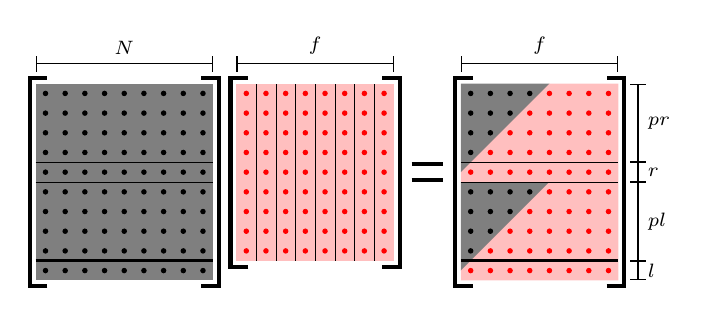
\begin{tikzpicture}
    % defining constants
    \def\stepSize{0.25}
    \def\Nnum{9}
    \def\fnum{8}
    \def\pnum{4}
    
    % Defining lengths
    \newlength{\onelen}
    \setlength{\onelen}{\stepSize cm}
    \newlength{\BrCl}
    \setlength{\BrCl}{0.075cm}
    \newlength{\BrIn}
    \setlength{\BrIn}{0.15cm}
    \newlength{\plen}
    \setlength{\plen}{1cm}%{\pnum\stepSize cm}
    \newlength{\flen}
    \setlength{\flen}{2cm}%{\fnum*\stepSize cm}
    \newlength{\Nlen}
    \setlength{\Nlen}{2.25cm}%{\Nnum\stepSize cm}%should be 2*p+one
    \newlength{\MatClearance}
    \setlength{\MatClearance}{0.3cm}
    
    % grid lines for guidance
    % \draw[gray,step=0.5] (-0,-1) grid (9,3);

    % ======================= drawing data matrix =======================
    \path (0,-\onelen) coordinate (M1A);
    \path ([xshift=\Nlen]M1A) coordinate (M1B);
    \path ([yshift=2*\plen+2*\onelen]M1B) coordinate (M1C);
    \path ([xshift=-\Nlen]M1C) coordinate (M1D);
    \draw[line width=1.5pt] ([xshift=\BrIn,yshift=-\BrCl]M1A) -- ([xshift=-\BrCl,yshift=-\BrCl]M1A) -- ([xshift=-\BrCl,yshift=\BrCl]M1D) -- ([xshift=\BrIn,yshift=\BrCl]M1D); %left bracket
    \draw[line width=1.5pt] ([xshift=-\BrIn,yshift=-\BrCl]M1B) -- ([xshift=\BrCl,yshift=-\BrCl]M1B) -- ([xshift=\BrCl,yshift=\BrCl]M1C) -- ([xshift=-\BrIn,yshift=\BrCl]M1C); %right bracket
    \draw[line width=1pt] ([yshift=\onelen]M1A) -- ([yshift=\onelen]M1B); % dividing matrix into blocks
    \fill[black, opacity=0.5] (M1A) rectangle (M1C);
    \foreach \x in {0,...,8} { % drawing black dots
    \foreach \y in {-1,...,8} {
      \fill ( {(\x+0.5)*\onelen}, {(\y+0.5)*\onelen} ) circle (1pt);
    }}
    \draw[line width=0.1pt] ([yshift=-\plen-\onelen]M1D) -- ([yshift=-\plen-\onelen]M1C);
    \draw[line width=0.1pt] ([yshift=-\plen]M1D) -- ([yshift=-\plen]M1C);
    
    % ======================= drawing G =======================
    % useful coordinates
    \path ([xshift=\MatClearance,yshift=\onelen]M1B) coordinate (M2A);
    \path ([xshift=\flen]M2A) coordinate (M2B);
    \path ([yshift=\Nlen]M2B) coordinate (M2C);
    \path ([xshift=-\flen]M2C) coordinate (M2D);

    % brackets
    \draw[line width=1.5pt] ([xshift=\BrIn,yshift=-\BrCl]M2A) -- ([xshift=-\BrCl,yshift=-\BrCl]M2A) -- ([xshift=-\BrCl,yshift=\BrCl]M2D) -- ([xshift=\BrIn,yshift=\BrCl]M2D); %left bracket
    \draw[line width=1.5pt] ([xshift=-\BrIn,yshift=-\BrCl]M2B) -- ([xshift=\BrCl,yshift=-\BrCl]M2B) -- ([xshift=\BrCl,yshift=\BrCl]M2C) -- ([xshift=-\BrIn,yshift=\BrCl]M2C); %right bracket
    
    % red fill
    \fill[red!50,opacity=0.5] (M2A) rectangle (M2C);

    % drawing red dots
    \foreach \x in {0,...,7} {
    \foreach \y in {0,...,8} {
      \fill[red] ([xshift=(\x+0.5)*\onelen,yshift=(\y+0.5)*\onelen]M2A) circle (1pt);%{(\x+0.5)*\onelen+\Nlen+0.5cm}, {(\y+0.5)*\onelen}
    }}

    % dividers
    \foreach \x in {1,...,7}{\draw[line width=0.1pt] ([xshift=\x*\onelen]M2A) -- ([xshift=\x*\onelen]M2D);}
    
    % ======================= drawing equal sign ======================= 
    \path ([xshift=\MatClearance*3/4,yshift=\Nlen/2-0.1cm]M2B) coordinate (EqA);
    \path ([xshift=0.4cm]EqA) coordinate (EqB);
    \path ([yshift=0.2cm]EqB) coordinate (EqC);
    \path ([xshift=-0.4cm]EqC) coordinate (EqD);
    \draw[line width = 1.5 pt] (EqA) -- (EqB);
    \draw[line width = 1.5 pt] (EqD) -- (EqC);

    % ======================= drawing RHS =======================
    % inside of matrix
    \path ([xshift=\MatClearance*3/4,yshift=-\Nlen/2+0.1cm-\onelen]EqB) coordinate (M3A);
    \path ([xshift=\flen]M3A) coordinate (M3B);
    \path ([yshift=2*\plen+2*\onelen]M3B) coordinate (M3C);
    \path ([xshift=-\flen]M3C) coordinate (M3D);
    % top left black triangle
    \path ([yshift=-\plen-\onelen/2]M3D) coordinate (t1A);
    \path ([xshift=\plen+\onelen/2]M3D) coordinate (t1B);
    % top red trapezoid
    \path ([yshift=-\onelen/2]t1A) coordinate (t2A);
    \path ([xshift=\flen]t2A) coordinate (t2B);
    % bottom black triangle
    \path ([yshift=-\plen-\onelen/2]t2A) coordinate (t3A);
    \path ([xshift=\plen+\onelen/2]t2A) coordinate (t3B);
    % bottom red trapezoid
    \path ([yshift=-\onelen/2]t3A) coordinate (t4A);

    % fill figures
    \fill[black, opacity=0.5]  (t1A) -- (t1B) -- (M3D) -- cycle;% top black
    \fill[red!50, opacity=0.5] (t2A) -- (t2B) -- (M3C) -- (t1B) -- (t1A) -- cycle;% top red
    \fill[black, opacity=0.5]  (t3A) -- (t3B) -- (t2A) -- cycle;% bottom black
    \fill[red!50, opacity=0.5] (t4A) -- (M3B) -- (t2B) -- (t3B) -- (t3A) -- cycle; % bottom red
    
    % draw brackets
    \draw[line width=1.5pt] ([xshift=\BrIn,yshift=-\BrCl]M3A) -- ([xshift=-\BrCl,yshift=-\BrCl]M3A) -- ([xshift=-\BrCl,yshift=\BrCl]M3D) -- ([xshift=\BrIn,yshift=\BrCl]M3D); %left bracket
    \draw[line width=1.5pt] ([xshift=-\BrIn,yshift=-\BrCl]M3B) -- ([xshift=\BrCl,yshift=-\BrCl]M3B) -- ([xshift=\BrCl,yshift=\BrCl]M3C) -- ([xshift=-\BrIn,yshift=\BrCl]M3C); %right bracket
    \draw[line width=1pt] ([yshift=\onelen]M3A) -- ([yshift=\onelen]M3B);
    
    % U_{i,p,N}
    \path ([xshift=0.5*\onelen,yshift=-\plen+0.5*\onelen]M3D) coordinate (tlbA);
    \foreach \x in {0,...,7}{
    \foreach \y in {0,...,3}{
        \ifthenelse{{\y>\x}\OR{\y=\x}}{%
        \fill[black] ([xshift={\x*\onelen},yshift={\y*\onelen}]tlbA) circle (1pt);%<do this if true>
        }{%
        \fill[red] ([xshift={\x*\onelen},yshift={(\y*\onelen}]tlbA) circle (1pt);%<do this if false>
        }%
    }}
    
    % U_{i_p,1,N}
    \path ([yshift=-\onelen]tlbA) coordinate (tlbB);
    \foreach \x in {0,...,7}{\fill[red] ([xshift=\x*\onelen]tlbB) circle (1pt);}
    
    % Y_{i,p,N}
    \path ([yshift=-\plen]tlbB) coordinate (tlbC);
    \foreach \x in {0,...,7}{
    \foreach \y in {0,...,3}{
        \ifthenelse{{\y>\x}\OR{\y=\x}}{%
        \fill[black] ([xshift={\x*\onelen},yshift={\y*\onelen}]tlbC) circle (1pt);%<do this if true>
        }{%
        \fill[red] ([xshift={\x*\onelen},yshift={(\y*\onelen}]tlbC) circle (1pt);%<do this if false>
        }%
    }}

    % Y_{i_p,1,N}
    \path ([yshift=-\onelen]tlbC) coordinate (tlbD);
    \foreach \x in {0,...,7}{\fill[red] ([xshift=\x*\onelen]tlbD) circle (1pt);}

    % draw dividers
    \draw[line width=0.1pt] ([yshift=-\plen-\onelen]M3D) -- ([yshift=-\plen-\onelen]M3C);
    \draw[line width=0.1pt] ([yshift=-\plen]M3D) -- ([yshift=-\plen]M3C);

    % ======================= length indicators ======================= 
    \draw[|-|] ([yshift=\onelen]M1D) -- node[above] {\scriptsize$N$} ([yshift=\onelen]M1C);
    \draw[|-|] ([yshift=\onelen]M2D) -- node[above] {\scriptsize$f$} ([yshift=\onelen]M2C);
    \draw[|-|] ([yshift=\onelen]M3D) -- node[above] {\scriptsize$f$} ([yshift=\onelen]M3C);
    \draw[|-|] ([xshift=\onelen]M3C) -- node[right] {\scriptsize$pr$} ([xshift=\onelen,yshift=\onelen]t2B);
    \draw[|-|] ([xshift=\onelen,yshift=\onelen]t2B) -- node[right] {\scriptsize$r$} ([xshift=\onelen]t2B);
    \draw[|-|] ([xshift=\onelen]t2B) -- node[right] {\scriptsize$pl$} ([xshift=\onelen,yshift=\onelen]M3B);
    \draw[|-|] ([xshift=\onelen,yshift=\onelen]M3B) -- node[right] {\scriptsize$l$} ([xshift=\onelen]M3B);
\end{tikzpicture}
\caption{Visualization of known (black) and unknown (red) variables in \ac{CL-DeePC} without \ac{IVs}. Each dot represents an input $u_k\in\mathbb{R}^r$, output $y_k\in\mathbb{R}^l$, or element of the matrix $G$. \ac{CL-DeePC} involves $f$ sequential applications of a step-ahead predictor obtained from regular \ac{DeePC} with $f=1$ (see also Fig.~\ref{fig:regular-DeePC}), resulting in the dashed block-anti diagonals with the same $u_k$ or $y_k$ on the right hand side.}
\label{fig:CL-DeePC}
\end{figure}
\begin{figure}[b!]
\centering
\begin{tikzpicture}
    % defining constants
    \def\stepSize{0.25}
    \def\Nnum{9}
    \def\fnum{8}
    \def\pnum{4}
    
    % Defining lengths
    % \newlength{\onelen}
    \setlength{\onelen}{\stepSize cm}
    % \newlength{\BrCl}
    \setlength{\BrCl}{0.075cm}
    % \newlength{\BrIn}
    \setlength{\BrIn}{0.15cm}
    % \newlength{\plen}
    \setlength{\plen}{1cm}%{\pnum\stepSize cm}
    % \newlength{\flen}
    \setlength{\flen}{2cm}%{\fnum*\stepSize cm}
    % \newlength{\Nlen}
    \setlength{\Nlen}{2.25cm}%{\Nnum\stepSize cm}%should be 2*p+one
    % \newlength{\MatClearance}
    \setlength{\MatClearance}{0.3cm}
    
    % grid lines for guidance
    % \draw[gray,step=0.5] (-0,-7) grid (8,3);

    % ======================= drawing data matrix =======================
    \path (0,2\plen+\onelen) coordinate (M1D);
    \path ([yshift=-2\plen-2\flen]M1D) coordinate (M1A);
    \path ([xshift=\Nlen]M1A) coordinate (M1B);
    \path ([yshift=2*\plen+2*\flen]M1B) coordinate (M1C);
    \draw[line width=1.5pt] ([xshift=\BrIn,yshift=-\BrCl]M1A) -- ([xshift=-\BrCl,yshift=-\BrCl]M1A) -- ([xshift=-\BrCl,yshift=\BrCl]M1D) -- ([xshift=\BrIn,yshift=\BrCl]M1D); %left bracket
    \draw[line width=1.5pt] ([xshift=-\BrIn,yshift=-\BrCl]M1B) -- ([xshift=\BrCl,yshift=-\BrCl]M1B) -- ([xshift=\BrCl,yshift=\BrCl]M1C) -- ([xshift=-\BrIn,yshift=\BrCl]M1C); %right bracket
    \draw[line width=1pt] ([yshift=\flen]M1A) -- ([yshift=\flen]M1B); % dividing matrix into blocks
    \fill[black, opacity=0.5] (M1A) rectangle (M1C);
    \foreach \x in {0,...,8} { % drawing black dots
    \foreach \y in {-15,...,8} {
      \fill ( {(\x+0.5)*\onelen}, {(\y+0.5)*\onelen} ) circle (1pt);
    }}
    \draw[line width=0.1pt] ([yshift=-\plen-\flen]M1D) -- ([yshift=-\plen-\flen]M1C);
    \draw[line width=0.1pt] ([yshift=-\plen]M1D) -- ([yshift=-\plen]M1C);

    % coordinates for diagonals
    \path ([yshift=-\plen]M1D) coordinate (M1stair1A);
    \path ([xshift=\Nlen]M1D) coordinate (M1stair1I);
    % black diagonals
    % \foreach \i in {0,-1}{
    % \foreach \dy in {1,...,18}{
    % \ifthenelse{\dy<9.5}{
    % % This code will be executed if \dy<9.5
    %     \draw[dash pattern=on 1pt off 2pt, line width=0.1pt] ([xshift= 0.5*\onelen,yshift=\i*(\plen+\flen)-(\dy+0.5)*\onelen]M1D) -- ([xshift= (\dy+0.5)*\onelen,yshift=\i*(\plen+\flen)-0.5*\onelen]M1D);
    % }{
    % % This code will be executed if \dy>=10
    %     \ifthenelse{\dy<12.5}{
    %         % This code will be executed if \dy<=12
    %         \draw[dash pattern=on 1pt off 2pt, line width=0.1pt] ([xshift= 0.5*\onelen,yshift=\i*(\plen+\flen)-(\dy+0.5)*\onelen]M1D) -- ([xshift= -0.5*\onelen,yshift=\i*(\plen+\flen)-(\dy-7.5)*\onelen]M1C);
    %         }{
    %         % This code will be executed if \dy>=13
    %         \draw[dash pattern=on 1pt off 2pt, line width=0.1pt] ([xshift= (\dy-10.5)*\onelen,yshift=\i*(\plen+\flen)-\plen-\flen+0.5*\onelen]M1D) -- ([xshift= -0.5*\onelen,yshift=\i*(\plen+\flen)-(\dy-7.5)*\onelen]M1C);
    %     }
    % }
    % }}
    
    % ---------------- drawing left brace and matrix ----------------
    \path ([xshift=-0.5\BrIn,yshift=-2\BrCl]M1A) coordinate (Brace1L);
    \path ([xshift=0.5\BrIn,yshift=-2\BrCl]M1B) coordinate (Brace1R);
    \draw[decorate, decoration={calligraphic brace, amplitude=3pt, mirror, aspect=0.75},line width=1pt] (Brace1L) -- (Brace1R);
    \node (mat1) at ($(Brace1L)!0.75!(Brace1R) + (0,-3pt)$) {};
    \node[below] at (mat1.center) {$\begin{bmatrix}
        U_{i,p,N}\\U_{i_p,f,N}\\Y_{i,p,N}\\ \hline Y_{i_p,f,N}
    \end{bmatrix}$};
    % brace to the left
    \path ([xshift=-0.75cm-0.05cm,yshift=-4pt]mat1.center) coordinate (Brace1T);
    \path ([yshift=-1.73cm]Brace1T) coordinate (Brace1B);
    \draw[pen colour=gray!60,decorate, decoration={calligraphic brace, amplitude=3pt, mirror, aspect=0.2},line width=0.75pt] (Brace1T) -- (Brace1B);
    % Zp
    \node (Zp) at ($(Brace1T)!0.2!(Brace1B) + (-3pt,-0.8pt)$) {};
    \node[left,text=gray!100,align=center] at ([xshift=0.5mm,yshift=-0.18cm]Zp.center) {\scriptsize{\shortstack{$=$\\$\Phi_{i,f,N}$}}};
  
    % ======================= drawing G =======================
    % useful coordinates
    \path ([xshift=\MatClearance,yshift=-0.5\Nlen-\plen-\flen]M1C) coordinate (M2A);
    \path ([xshift=\onelen]M2A) coordinate (M2B);
    \path ([yshift=\Nlen]M2B) coordinate (M2C);
    \path ([xshift=-\onelen]M2C) coordinate (M2D);

    % brackets
    \draw[line width=1.5pt] ([xshift=0.5\BrIn,yshift=-\BrCl]M2A) -- ([xshift=-\BrCl,yshift=-\BrCl]M2A) -- ([xshift=-\BrCl,yshift=\BrCl]M2D) -- ([xshift=0.5\BrIn,yshift=\BrCl]M2D); %left bracket
    \draw[line width=1.5pt] ([xshift=-0.5\BrIn,yshift=-\BrCl]M2B) -- ([xshift=\BrCl,yshift=-\BrCl]M2B) -- ([xshift=\BrCl,yshift=\BrCl]M2C) -- ([xshift=-0.5\BrIn,yshift=\BrCl]M2C); %right bracket
    
    % red fill
    \fill[red!50,opacity=0.5] (M2A) rectangle (M2C);

    % drawing red dots
    \foreach \x in {0} {
    \foreach \y in {0,...,8} {
      \fill[red] ([xshift=(\x+0.5)*\onelen,yshift=(\y+0.5)*\onelen]M2A) circle (1pt);
    }}

    % drawing middle brace and matrix
    \coordinate (Brace2L) at ([xshift=-0.5\BrIn]M2A |- Brace1L);
    \coordinate (Brace2R) at ([xshift=0.5\BrIn]M2B |- Brace1L);
    \draw[decorate, decoration={calligraphic brace, amplitude=3pt, mirror, aspect=0.5},line width=1pt] (Brace2L) -- (Brace2R);
    \node (mat1) at ($(Brace2L)!0.5!(Brace2R) + (0,-3pt)$) {};
    \node[below] at ([yshift=-1.05cm]mat1.center) {$g$};
    
    % ======================= drawing equal sign ======================= 
    \path ([xshift=\MatClearance*3/4,yshift=\Nlen/2-0.1cm]M2B) coordinate (EqA);
    \path ([xshift=0.4cm]EqA) coordinate (EqB);
    \path ([yshift=0.2cm]EqB) coordinate (EqC);
    \path ([xshift=-0.4cm]EqC) coordinate (EqD);
    \draw[line width = 1.5 pt] (EqA) -- (EqB);
    \draw[line width = 1.5 pt] (EqD) -- (EqC);

    % ---------------- equation sign below ----------------
    \node[below] at ([xshift=2\onelen,yshift=-1.05cm]mat1.center) {$=$};

    % ======================= drawing RHS =======================
    % inside of matrix
    \path ([xshift=0.75\MatClearance]EqB |- M1A) coordinate (M3A);
    \path ([xshift=\onelen]M3A) coordinate (M3B);
    \path ([yshift=2\plen+2\flen]M3B) coordinate (M3C);
    \path ([xshift=-\onelen]M3C) coordinate (M3D);
    
    % fill figures
    \fill[black,opacity=0.5]  (M3D) -- ([yshift=-\plen]M3D) -- ([yshift=-\plen]M3C) -- (M3C) -- cycle;
    \fill[red!50,opacity=0.5] ([yshift=-\plen]M3D) -- ([yshift=-\plen-\flen]M3D) -- ([yshift=-\plen-\flen]M3C) -- ([yshift=-\plen]M3C) -- cycle;
    \fill[black,opacity=0.5] ([yshift=\flen]M3A) -- ([yshift=\flen]M3B) -- ([yshift=\flen+\plen]M3B) -- ([yshift=\flen+\plen]M3A) -- cycle;
    \fill[red!50,opacity=0.5]  (M3A) -- (M3B) -- ([yshift=\flen]M3B) -- ([yshift=\flen]M3A) -- cycle;
    
    % draw brackets
    \draw[line width=1.5pt] ([xshift=0.5\BrIn,yshift=-\BrCl]M3A) -- ([xshift=-\BrCl,yshift=-\BrCl]M3A) -- ([xshift=-\BrCl,yshift=\BrCl]M3D) -- ([xshift=0.5\BrIn,yshift=\BrCl]M3D); %left bracket
    \draw[line width=1.5pt] ([xshift=-0.5\BrIn,yshift=-\BrCl]M3B) -- ([xshift=\BrCl,yshift=-\BrCl]M3B) -- ([xshift=\BrCl,yshift=\BrCl]M3C) -- ([xshift=-0.5\BrIn,yshift=\BrCl]M3C); %right bracket
    
    % U_{i,p,1}
    \foreach \dy in {0,...,-3}{
        \fill[black] ([xshift=0.5\onelen,yshift=(\dy-0.5)*\onelen]M3D) circle (1pt);
    }

    % U_{i_p,f,1}
    \foreach \dy in {-4,...,-11}{
        \fill[red] ([xshift=0.5\onelen,yshift=(\dy-0.5)*\onelen]M3D) circle (1pt);
    }
    
    % Y_{i,p,1}
    \foreach \dy in {0,...,-3}{
        \fill[black] ([xshift=0.5\onelen,yshift=(\dy-0.5)*\onelen-\plen-\flen]M3D) circle (1pt);
    }

    % Y_{i_p,f,1}
    \foreach \dy in {-4,...,-11}{
        \fill[red] ([xshift=0.5\onelen,yshift=(\dy-0.5)*\onelen-\plen-\flen]M3D) circle (1pt);
    }

    % draw dividers
    \draw[line width=0.1pt] ([yshift=-\plen]M3D) -- ([yshift=-\plen]M3C);
    \draw[line width=0.1pt] ([yshift=-\plen-\flen]M3D) -- ([yshift=-\plen-\flen]M3C);
    \draw[line width=1pt] ([yshift=\flen]M3A) -- ([yshift=\flen]M3B);

    % ---------------- drawing right brace and matrix ----------------
    % brace below matrix
    \path ([xshift=-0.5\BrIn,yshift=-2\BrCl]M3A) coordinate (Brace3L);
    \path ([xshift=0.5\BrIn,yshift=-2\BrCl]M3B) coordinate (Brace3R);
    \draw[decorate, decoration={calligraphic brace, amplitude=3pt, mirror, aspect=0.5},line width=1pt] (Brace3L) -- (Brace3R);
    % matrix below brace
    \node (mat3) at ($(Brace3L)!0.5!(Brace3R) + (0,-3pt)$) {};
    \node[below] at ([xshift=0.35cm]mat3.center) {$\begin{bmatrix}
        U_{\hat{i},p,1}\\U_{\hat{i}_p,f,1}\\Y_{\hat{i},p,1}\\ \hline Y_{\hat{i}_p,f,1}
    \end{bmatrix}$};
    % tag & label (on RHS of column)
    \node[below left] at (8.35cm,-5cm) {$\refstepcounter{equation}(\theequation)\label{eq:regular_DeePC_no_IVs}$};
    % brace to the right
    \path ([xshift=1.1cm]mat3.center |- Brace1T) coordinate (Brace3T);%([xshift=0.7cm,yshift=-4pt]mat3.center) coordinate (Brace3T);
    \path (Brace3T |- Brace1B) coordinate (Brace3B);
    \draw[pen colour=gray!60,decorate, decoration={calligraphic brace, amplitude=3pt, aspect=0.2},line width=0.75pt] (Brace3T) -- (Brace3B);
    % Zf
    \node (Zf) at ($(Brace3T)!0.2!(Brace3B) + (3pt,-1.5pt)$) {};
    \node[right,text=gray!100] at ([yshift=-0.18cm]Zf.center) {\scriptsize{\shortstack{$=$\\$\Phi_{\hat{i},f,1}$}}};
    
    % ======================= length indicators ======================= 
    \draw[|-|] ([yshift=\onelen]M1D) -- node[above] {\scriptsize$N$} ([yshift=\onelen]M1C);
    \draw[|-|] ([xshift=\onelen]M3C) -- node[right] {\scriptsize$pr$} ([xshift=\onelen,yshift=-\plen]M3C);
    \draw[|-|] ([xshift=\onelen,yshift=-\plen]M3C) -- node[right] {\scriptsize$fr$} ([xshift=\onelen,yshift=-\plen-\flen]M3C);
    \draw[|-|] ([xshift=\onelen,yshift=-\plen-\flen]M3C) -- node[right] {\scriptsize$pl$} ([xshift=\onelen,yshift=\flen]M3B);
    \draw[|-|] ([xshift=\onelen,yshift=\flen]M3B) -- node[right] {\scriptsize$fl$} ([xshift=\onelen]M3B);
\end{tikzpicture}
\caption{Visualization of known (black) and unknown (red) variables in \ac{DeePC} without \ac{IVs}. Each dot represents an input $u_k\in\mathbb{R}^r$, output $y_k\in\mathbb{R}^l$, or element of the matrix $G$. A multi-step ahead predictor of prediction length $f$ is formed directly by taking a linear combination of past input and output data.\\\vspace{0.75mm}}
\label{fig:regular-DeePC}
\end{figure}
%
\setcounter{thm}{0}
\begin{thm}\label{theorem:main_result}
    Consider the minimal discrete non-deterministic \ac{LTI} system given by~\eqref{eqn:SS_innovation} to generate input-output data in closed-loop by means of a causal controller without direct feedthrough, and data matrices $\overline{\Psi}_{\hat{i},1,f}$ and $\Psi_{i,1,N_\mathrm{s}}$ as in \eqref{eq:Phi_def}. If $N_\mathrm{s}=(p+1)r+pl$ such that $\Psi_{i,1,N_\mathrm{s}}$ is square, and furthermore, if $\Psi_{i,1,N_\mathrm{s}}$ is invertible, %
    %
    % If the joint input and noise sequences are sufficiently persistently exciting such that $\left[X_{i,1,N}^\top \; U_{i,p,N}^\top \; U_{i_p,1,N}^\top \; E_{i,p,N}^\top\right]^\top$ is full row rank %
    % ------------------------------------------------------
    %% ----------------- old version below -----------------
    %If the input sequence $\{u_k\}_{k=i}^{i+\bar{N}-1}$ of length $\bar{N}=p+s+N-1$ %, with $N\geq(p+s+n)(r+l)+n$ and $p\geq\ell$\todo{don't forget},
    % is persistently exciting of order $p+s+n$, and has sample correlations such that%
    % \begin{alignat}{2}%see also https://www.cis.upenn.edu/~jean/schur-comp.pdf
    % % \widehat{\Sigma}_{u,u} &> 0,\label{eq:PE_corU}\\
    % &\widehat{\Sigma}_{\mathrm{ee}} - \widehat{\Sigma}_{\mathrm{ue}^\top} \widehat{\Sigma}_{\mathrm{uu}}\inv \widehat{\Sigma}_{\mathrm{ue}}\succ0,\span\span\label{eq:PE_corUE2}\\
    % &&\text{with}\quad\widehat{\Sigma}_{\mathrm{ee}}&=E_{i,p+s+n,N-n}E_{i,p+s+n,N-n}^\top,\notag\\
    % &&\widehat{\Sigma}_{\mathrm{ue}}&=U_{i,p+s+n,N-n}E_{i,p+s+n,N-n}^\top,\notag\\
    % &&\widehat{\Sigma}_{\mathrm{uu}}&=U_{i,p+s+n,N-n}U_{i,p+s+n,N-n}^\top,\notag
    % \end{alignat}
    % ------------------------------------------------------
    then \\
    $\mathrm{(i)}$ $\exists G\in\mathbb{R}^{N\times f}$ such that
    \begin{align}\tag{\ref{eq:CL_DeePC_no_IVs}}%\label{eq:Theorem1}
        \begin{bmatrix}
            \Psi_{i,1,N_\mathrm{s}}\\
            Y_{i_p,1,N_\mathrm{s}}
        \end{bmatrix}G =
        \begin{bmatrix}
            \overline{\Psi}_{\hat{i},1,f}\\
            \widehat{Y}_{\hat{i}_p,1,f}
        \end{bmatrix},
    \end{align}
    $\mathrm{(ii)}$ and with $\widehat{Y}_{\hat{i}_p,1,f}$ as an asymptotically unbiased predictor %with respect to both past and future noise 
    with respect to future noise and conditioned on past data as $p\rightarrow\infty$.\todo{Compa-rative rates?\\also
    $N_\mathrm{s}\rightarrow\infty$}%
\end{thm}

\subsection{Auxiliary results}
The proof of Theorem~\ref{theorem:main_result} is deferred till after the treatment of several auxiliary results. The first of which is the following lemma.
\setcounter{thm}{0}
\begin{lem}\label{lem:relative_rates}\citep{Bauer2002,Chiuso2006}
    A necessary condition for consistent closed-loop subspace identification is that as $p\rightarrow\infty$, $N\rightarrow\infty$ such that
    \begin{align}\label{eq:relative_rates}
        \begin{split}
            p &\geq -\frac{d\log N}{2\log|\rho|}, \quad 1 < d < \infty,\\
            \lim_{p,N\rightarrow\infty} &\; \frac{p}{(\log N)^\alpha}=0, \quad \alpha < \infty,
        \end{split}
    \end{align}
\end{lem}
where $\rho$ is the eigenvalue of $\tilde{A}$ of maximum modulus.

\begin{lem}\label{lem:oblique_projections}\citep[Lemma~1]{VanOverschee1994,Katayama1999} Let $a$, $b$ and $c$ be random vectors with components in the Hilbert space $\mathscr{H}$, $\mathscr{A}=\text{span}\{a\}$, $\mathscr{B}=\text{span}\{b\}$ and $\mathscr{A}\cap\mathscr{B}=\{0\}$. Furthermore, let correlation matrices be exemplified by $\Sigma_{ca}=\mathbb{E}[ca^\top]$ and their conditional counterparts by $\Sigma_{ca|b}=\mathbb{E}[(c|b^\bot)(a|b^\bot)^\top]$, with $\bot$ denoting the orthogonal complement. Then the orthogonal projection of the row space of $c$ on the joint row space of $a$ and $b$ is the sum of the oblique projections $\Pi_{ca||b}a$ ($c$ onto $\mathscr{A}$ along $\mathscr{B}$) and $\Pi_{cb||a}b$ ($c$ onto $\mathscr{B}$ along $\mathscr{A}$) as
\begin{align}
    \begin{bmatrix}
        \Sigma_{ca} & \Sigma_{cb}
    \end{bmatrix}
    \begin{bmatrix}
        \Sigma_{aa} & \Sigma_{ab}\\ \Sigma_{ba} & \Sigma_{bb}
    \end{bmatrix}^\dagger
    \begin{bmatrix}
        a \\ b
    \end{bmatrix} = \Pi_{ca||b} a + \Pi_{cb||a} b,\label{eq:oblique_project}\\
    \text{s.t. }\quad\Pi_{ca||b}\Sigma_{aa|b} = \Sigma_{ca|b},\quad \Pi_{cb||a}\Sigma_{bb|a} = \Sigma_{cb|a}.\notag
\end{align}
The conditional correlation matrices may be expressed as demonstrated by $\Sigma_{ca|b}=\Sigma_{ca}-\Sigma_{cb}\Sigma_{bb}\inv\Sigma_{ba}$ if the involved inverse exists. In addition, $\Sigma_{aa|b}$ and $\Sigma_{bb|a}$ are invertible if $\Sigma_{aa}$ and $\Sigma_{bb}$ are invertible.
\end{lem}
\subsection{Proof of Theorem~\ref{theorem:main_result}}
% ---------------- Proof of (i) ----------------
\noindent\textbf{Proof of $(\mathrm{i})$:} In \eqref{eq:CL_DeePC_no_IVs} the output predictor is an optimization variable that is defined in terms of $G$, leaving its top matrix equations to specify $G$ as
\begin{align}\label{eq:G_sols}
    G = \Psi_{i,1,N_\mathrm{s}}^{\dagger,\mathrm{r}}\overline{\Psi}_{\hat{i},1,f} = \Psi_{i,1,N_\mathrm{s}}\inv\overline{\Psi}_{\hat{i},1,f},
\end{align}
in which, by definition, of the right inverse, $\Psi_{i,1,N_\mathrm{s}}^{\dagger,\mathrm{r}}=\Psi_{i,1,N_\mathrm{s}}^\top \left(\Psi_{i,1,N_\mathrm{s}}\Psi_{i,1,N_\mathrm{s}}^\top\right)\inv$. Since $\Psi_{i,1,N_\mathrm{s}}$ is square and invertible this reduces to $\Psi_{i,1,N_\mathrm{s}}\inv$. The solution to $G$ provided by \eqref{eq:G_sols} proves that $\exists G$ that satisfies \eqref{eq:CL_DeePC_no_IVs}. $\hfill\qed$
% 
% Decomposing $\Psi_{i,1,N}$ into its dependencies begets
% \begin{align}\label{eq:Phi_isN}
%     \mkern-8mu\Psi_{i,1,N}=\mkern-1mu\begin{bmatrix}
%         U_{i,p,N}\\
%         U_{i_p,1,N}\\
%         Y_{i,p,N}
%     \end{bmatrix}\mkern-1mu=\mkern-1mu
%     \underbrace{\begin{bmatrix}
%         0        & I_{pr} & 0      & 0\\
%         0        & 0      & I_{r} & 0\\
%         \Gamma_p & \mathcal{T}_p^\mathrm{u} & 0 & \mathcal{H}_p
%     \end{bmatrix}}\mkern-3mu\begin{bmatrix}
%         X_{i,1,N}\\
%         U_{i,p,N}\\
%         U_{i_p,1,N}\\
%         E_{i,p,N}
%     \end{bmatrix}\mkern-1mu,
% \end{align}
% in which the matrix on the right hand side is assumed to be full row rank, and the underbraced matrix is also full row rank. Since both of these matrices are full row rank, so is its product $\Psi_{i,1,N}$, meaning that there exists at least one $G$ that satisfies \eqref{eq:CL_DeePC_no_IVs}. 

% \noindent\textbf{Remark 1:} For the matrix on the right hand side of \eqref{eq:Phi_isN} to be guaranteed to be of full row rank a necessary condition is that $N\geq n+(p+1)r+pl$.

% \noindent\textbf{Remark 2:} The full row rank matrix $\Psi_{i,1,N}\in\mathbb{R}^{((p+1)r+pl)\times N}$ has more columns than rows, meaning that in fact there are an infinite number of possibilities for $G$ that satisfy \eqref{eq:CL_DeePC_no_IVs}. These possibilities are given by
% % \begin{align}\label{eq:G_sols}
% %     G = \Psi_{i,1,N}^\dagger\overline{\Psi}_{\hat{i},1,f} + \Pi_{\Psi_{i,1,N}}^\bot W,
% % \end{align}
% in which the dagger $\dagger$ denotes the right inverse ($\mathcal{Q}^\dagger=\mathcal{Q}^\top(\mathcal{Q}\mathcal{Q}^\top)\inv$ with $\mathcal{Q}$ as a real, full row rank matrix), $\Pi_{\Psi_{i,1,N}}^\bot=I_N-\Psi_{i,1,N}^\dagger\Psi_{i,1,N}$ is a projection matrix onto the orthogonal complement of the row space of $\Psi_{i,1,N}$, %see Overschee1996, pg. 19
% and $W\in\mathbb{R}^{N\times f}$ is a matrix of decision variables that parameterizes $G$.

% ---------------- Proof of (ii) ----------------
\noindent\textbf{Proof of $(\mathrm{ii})$:} Equation \eqref{eq:CL_DeePC_no_IVs} stipulates an output predictor as $\widehat{Y}_{\hat{i}_p,1,f}=Y_{i_p,1,N_\mathrm{s}}G$. %
Using \eqref{eq:DataEq1}, \eqref{eq:G_sols}, and considering $\Gamma_1=C$, $\mathcal{H}_1=I_l$, $L_1=\big[C\tKp{u} \;\;\! D \;\;\! C\tKp{y}\big]$ yields
\begin{align}
    \mkern-6mu\widehat{Y}_{\hat{i}_p,1,f} &= C \tilde{A}^p X_{i,1,N_\mathrm{s}}G + E_{i_p,1,N_\mathrm{s}}G + L_1 \Psi_{i,1,N_\mathrm{s}}G\notag\\
    \begin{split}
        &=\!\Big(\!\big(C \tilde{A}^p \underbrace{X_{i,1,N_\mathrm{s}}\Psi_{i,1,N_\mathrm{s}}^\top}_{=\hat{\Sigma}_{x\psi}} + \underbrace{E_{i_p,1,N_\mathrm{s}}\Psi_{i,1,N_\mathrm{s}}^\top}_{=\hat{\Sigma}_{e\psi}}\big)\times\\
        &\phantom{==}\big(\smash{\underbrace{\Psi_{i,1,N_\mathrm{s}}\Psi_{i,1,N_\mathrm{s}}^\top}_{=\hat{\Sigma}_{\psi\psi}}}\big)\inv+\begin{bmatrix}C\tKp{u} & D & C\tKp{y}\end{bmatrix}\Big)\overline{\Psi}_{\hat{i},1,f},
    \end{split}\label{eq:Yfhat_1}
\end{align}
in which the underbraced terms define the indicated sample correlation matrices. Partitioning the matrix $\Psi_{i,1,N_\mathrm{s}}=[U_{i,p+1,N_\mathrm{s}}^\top\;Y_{i,p,N_\mathrm{s}}^\top]^\top$ such that
\begin{alignat*}{3}
    \hat{\Sigma}_{\psi\psi}&=\begin{bmatrix}
        \hat{\Sigma}_{uu} & \hat{\Sigma}_{uy}\\
        \hat{\Sigma}_{yu} & \hat{\Sigma}_{yy}
    \end{bmatrix} &&= \begin{bmatrix} U_{i,p+1,N_\mathrm{s}} \\ Y_{i,p,N_\mathrm{s}} \end{bmatrix}\begin{bmatrix} U_{i,p+1,N_\mathrm{s}}^\top & Y_{i,p,N_\mathrm{s}}^\top \end{bmatrix},\\
    \hat{\Sigma}_{x\psi}&=\begin{bmatrix}
        \hat{\Sigma}_{xu} & \hat{\Sigma}_{xy}
    \end{bmatrix} &&= X_{i,1,N_\mathrm{s}}\begin{bmatrix} U_{i,p+1,N_\mathrm{s}}^\top & Y_{i,p,N_\mathrm{s}}^\top \end{bmatrix},\\
    \hat{\Sigma}_{e\psi}&=\begin{bmatrix}
        \hat{\Sigma}_{eu} & \hat{\Sigma}_{ey}
    \end{bmatrix} &&= E_{i_p,1,N_\mathrm{s}}\begin{bmatrix} U_{i,p+1,N_\mathrm{s}}^\top & Y_{i,p,N_\mathrm{s}}^\top \end{bmatrix},
\end{alignat*}
and applying Lemma~\ref{lem:oblique_projections}, \eqref{eq:Yfhat_1} is rewritten in terms of oblique sample projections as
\begin{align}\label{eq:Yfhat_2}
    \begin{split}
    \widehat{Y}_{\hat{i}_p,1,f} = \Big(C\tilde{A}^p\hat{\Pi}_{xy||u}+\hat{\Pi}_{ey||u}
    + C\tKp{y}\Big)&\overline{Y}_{\hat{i},p,f}\\
    +\Big(C\tilde{A}^p\hat{\Pi}_{xu||y}+\hat{\Pi}_{eu||y}+
    \begin{bmatrix}C\tKp{u} & D \end{bmatrix}\!\Big)&U_{\hat{i},p+1,f},
    \end{split}
\end{align}
with the sample-based oblique projection matrices
\begin{alignat*}{3}
    \hat{\Pi}_{xy||u}&=\hat{\Sigma}_{xy|u}\hat{\Sigma}_{yy|u}\inv, \qquad &\hat{\Pi}_{ey||u}&=\hat{\Sigma}_{ey|u}\hat{\Sigma}_{yy|u}\inv,\\
    \hat{\Pi}_{xu||y}&=\hat{\Sigma}_{xu|y}\hat{\Sigma}_{uu|y}\inv,        &\hat{\Pi}_{eu||y}&=\hat{\Sigma}_{eu|y}\hat{\Sigma}_{uu|y}\inv.
\end{alignat*}
Note that the invertibility of $\hat{\Sigma}_{yy|u}$ and $\hat{\Sigma}_{uu|y}$ is ensured according to Lemma~\ref{lem:oblique_projections} by the non-singularity of $\hat{\Sigma}_{yy}$ and $\hat{\Sigma}_{uu}$, which in turn derives from the full row rank of $\Psi_{i,1,N_\mathrm{s}}$.

Having derived the output predictor obtained from \eqref{eq:CL_DeePC_no_IVs}, now consider its error. Equations \eqref{eq:DataEq1} and \eqref{eq:Yfhat_2} determine this error as
%
%Consider the error of this prediction, which using \eqref{eq:DataEq1}, and considering $\Gamma_1=C$, $\mathcal{H}_1=I_l$ is written as
\begin{align}
    \begin{split}
        &\widehat{Y}_{\hat{i}_p,1,f}-Y_{\hat{i}_p,1,f} = C\tKp{y}\left(\overline{Y}_{\hat{i},p,f}-Y_{\hat{i},p,f}\right)\\
        &\;\;\;+C\tilde{A}^p\!\left(\hat{\Pi}_{xy||u}\overline{Y}_{\hat{i},p,f}+\hat{\Pi}_{xu||y} U_{\hat{i},p+1,f}-X_{\hat{i},1,f}\!\right)\\
        &\;\;\;+\hat{\Pi}_{eu||y}U_{\hat{i},p+1,f}+\hat{\Pi}_{ey||u}\overline{Y}_{\hat{i},p,f}-E_{\hat{i}_p,1,f}
    \end{split}\label{eq:Yf_error1}%\\
    % \begin{split}
    %     &\!\!\!\widehat{Y}_{\hat{i}_p,1,f}-Y_{\hat{i}_p,1,f} = C \tilde{A}^p (%\underbrace{
    %     X_{i,1,N_\mathrm{s}}G%}_{=\widehat{X}_{\hat{i},1,f}}
    %     -X_{\hat{i},1,f})-E_{\hat{i}_p,1,f}\\
    %     &\phantom{=}+ L_1(\smash{\underbrace{\Psi_{i,1,N_\mathrm{s}}G}_{\mathrlap{=\overline{\Psi}_{\hat{i},1,f}\;\because \text{ \eqref{eq:CL_DeePC_no_IVs}}}}}
    %     -\Psi_{\hat{i},1,f}) +%\underbrace{
    %     E_{i_p,1,N_\mathrm{s}}\underbrace{G}_{\mathclap{=\Psi_{i,1,N_\mathrm{s}}^{\dagger,\mathrm{r}}\overline{\Psi}_{\hat{i},1,f}\;\because\text{ \eqref{eq:G_sols}}}}%}_{=\widehat{E}_{\hat{i}_p,1,f}}
    % \end{split}\notag\\
    % \begin{split}
    %     &=C \tilde{A}^p (X_{i,1,N_\mathrm{s}}G-X_{\hat{i},1,f}) - E_{\hat{i}_p,1,f}\\
    %     &\phantom{=}+C\tKp{y}\left(\overline{Y}_{\hat{i},p,f}-Y_{\hat{i},p,f}\right)\\
    %     &\phantom{=}+\underbrace{E_{i_p,1,N_\mathrm{s}}\Psi_{i,1,N_\mathrm{s}}^\top}_{=\hat{\Sigma}_{e\psi}}(\underbrace{\Psi_{i,1,N_\mathrm{s}}\Psi_{i,1,N_\mathrm{s}}^\top}_{=\hat{\Sigma}_{\psi}})\inv \overline{\Psi}_{\hat{i},1,f},
    % \end{split}\label{eq:Yf_error1}
\end{align}
Applying the limit $p\rightarrow\infty$ asymptotically attenuates the error of the implicit initial state estimates on the second row since, by the definition of $K$ in \secref{sec:sys_model}, $\tilde{A}$ has all of its eigenvalues strictly inside the unit circle. Moreover, since $N_\mathrm{s}=(p+1)r+pl$, the limit $p\rightarrow\infty$ also ensures $N_\mathrm{s}\rightarrow\infty$. In this latter limit the sample correlation matrices approach their true correlation matrix with probability one because inputs and outputs are assumed to be quasi-stationary second-order ergodic stochastic processes. To this end, consider the sample correlation matrix $\hat{\Sigma}_{e\psi}$ that governs the oblique projection matrices $\hat{\Pi}_{eu||y}$ and $\hat{\Pi}_{ey||u}$ as indicated by \eqref{eq:oblique_project}.
\begin{align}\label{eq:E_Phi_correlation}
    \begin{split}
        &\hat{\Sigma}_{e\psi} = \\
        &\;\frac{1}{N_\mathrm{s}}\;\sum\limits_{k=i_p}^{\mathclap{i_p+N_\mathrm{s}-1}} e_k \begin{bmatrix}u_{k-p}^\top & \cdots & u_{k-1}^\top & u_k^\top & y_{k-p}^\top & \cdots & y_{k-1}^\top \end{bmatrix}.
    \end{split}
\end{align}
Due to the feedback of a (by assumption) strictly causal controller, inputs are correlated with preceding noise (${\mathbb{E}[e_k u_j^\top]\neq0,\; \forall j>k}$), but inputs are uncorrelated with concurrent and subsequent noise (${\mathbb{E}[e_k u_j^\top]=0,\; \forall j\leq k}$). Since the innovation noise is also uncorrelated with preceding outputs (${\mathbb{E}[e_k y_j^\top]=0,\; \forall j<k}$), there is no correlation between the relevant terms in \eqref{eq:E_Phi_correlation} and the expectation of the bottom row of \eqref{eq:Yf_error2} with respect to future noise is zero in the limit $p,N_\mathrm{s}\rightarrow\infty$.


\begin{alignat}{2}
\begin{split}\label{eq:Yf_error2}
    \!\!&\lim_{p\rightarrow\infty}\widehat{Y}_{\hat{i}_p,1,f}-Y_{\hat{i}_p,1,f} = \lim_{p\rightarrow\infty}\!\Big[C\tKp{y}\left(\overline{Y}_{\hat{i},p,f}-Y_{\hat{i},p,f}\right)\\
        &%+E_{i_p,1,N_\mathrm{s}} \Pi_{\Psi_{i,1,N_\mathrm{s}}}^\bot W
        \quad+\hat{\Pi}_{eu||y}U_{\hat{i},p+1,f}+\hat{\Pi}_{ey||u}\overline{Y}_{\hat{i},p,f}-E_{\hat{i}_p,1,f}\Big].
\end{split}
\end{alignat}%
Taking the expectation (denoted by $\mathbb{E}[\cdot]$) with respect to future noise as conditioned on past data (denoted by $\mathbb{E}^\mathrm{f}[\cdot]$) of \eqref{eq:Yf_error2} removes the dependence on future noise $E_{\hat{i}_p,1,f}$. Consider the correlation matrix
% For the predictor to be unbiased, the expectation (which we will denote with $\mathbb{E}[\cdot]$) of this error w.r.t. the noise must be zero. \todo{$\mathbb{E}[\cdot]$,\\$EW$,\\$\hat{\Sigma}\hat{\Sigma}\inv$?} Consider the underbraced correlation matrix
\begin{align}%\label{eq:E_Phi_correlation}
    \begin{split}
        &\hat{\Sigma}_{e\psi} = \\
        &\;\frac{1}{N_\mathrm{s}}\;\sum\limits_{k=i_p}^{\mathclap{i_p+N_\mathrm{s}-1}} e_k \begin{bmatrix}u_{k-p}^\top & \cdots & u_{k-1}^\top & u_k^\top & y_{k-p}^\top & \cdots & y_{k-1}^\top \end{bmatrix}.
    \end{split}
\end{align}
Since $N_\mathrm{s}=(p+1)r+pl$, the limit $p\rightarrow\infty$ also ensures $N_\mathrm{s}\rightarrow\infty$. By the assumed conditions of second-order ergodicity and quasi-stationarity, the correlation matrix of \eqref{eq:E_Phi_correlation} asymptotically approaches a well-defined true correlation matrix. Due to the feedback of a (by assumption) strictly causal controller, inputs are correlated with preceding noise (${\mathbb{E}[e_k u_j^\top]\neq0,\; \forall j>k}$), but inputs are uncorrelated with concurrent and subsequent noise (${\mathbb{E}[e_k u_j^\top]=0,\; \forall j\leq k}$). Since the innovation noise is also uncorrelated with preceding outputs (${\mathbb{E}[e_k y_j^\top]=0,\; \forall j<k}$), there is no correlation between the relevant terms in \eqref{eq:E_Phi_correlation} and the expectation of the bottom row of \eqref{eq:Yf_error2} with respect to future noise is zero in the limit $p,N_\mathrm{s}\rightarrow\infty$. %Since $E_{i_p,1,N}$ and $\Psi_{i,1,N}$ are uncorrelated, $\mathbb{E}[E_{i_p,1,N} \Pi_{\Psi_{i,1,N}}^\bot W]=\mathbb{E}[E_{i_p,1,N}W]=0$ such that the expectation of the second row of \eqref{eq:Yf_error2} is also zero.

Given the structure of $\overline{\Psi}_{\hat{i},1,f}$ and $\overline{Y}_{\hat{i},p,f}$ shown in Fig.~\ref{fig:CL-DeePC}, consider \eqref{eq:Yf_error2} column by column. As discussed, taking the expectation conditioned on past data leaves
\begin{align}\label{eq:Yf_error3}
\begin{split}
    &\mkern-3mu\lim_{p\rightarrow\infty} \mathbb{E}^\mathrm{f}\left[\hat{y}_{\hat{i}_p+k}-y_{\hat{i}_p+k}\right] = \\ &\;\;\;\lim_{p\rightarrow\infty}C\tKp{y}\mathbb{E}^\mathrm{f}\left[\datavec{\overline{y}}{\hat{i}+k,p}-\datavec{y}{\hat{i}+k,p}\right],\forall k\in[0,f-1].
\end{split}
\end{align}
By \eqref{eq:Yf_error3} in the limit $p\rightarrow\infty$ the prediction $\hat{y}_{\hat{i}_p+k}$ is unbiased if the $p$ preceding output estimates are unbiased. For $k=0$, this is the case because none of the relevant preceding output data is estimated ($\datavec{\overline{y}}{\hat{i},p}=\datavec{y}{\hat{i},p}$). No bias is thereby introduced on the right hand side for $k=1$ such that $\hat{y}_{\hat{i}_p+1}$ is also unbiased. Repetition of this process until $k=f-1$ demonstrates that, in the limit $p\rightarrow\infty$, $\widehat{Y}_{\hat{i}_p,1,f}$ is indeed an asymptotically unbiased predictor with respect to future noise and conditioned on past data. This concludes the proof of $\mathrm{(ii)}$. $\hfill\qed$

\subsection{Systematic noise mitigation using \ac{IVs}}
The previous section demonstrated that the predictor that is obtained from \eqref{eq:CL_DeePC_no_IVs} is asymptotically unbiased. This section demonstrates the use of \ac{IVs} as a means to decrease the variance of this predictor.

Since the relevant innovation and input-output samples in the correlation matrix of \eqref{eq:E_Phi_correlation} are uncorrelated, the underbraced term in \eqref{eq:Yf_error2} vanishes asymptotically as $N_\mathrm{s}\rightarrow\infty$. Since $N_\mathrm{s}=(p+1)r+pl$, the rate at which the underbraced term vanishes in \eqref{eq:Yf_error2} is determined by the rate at which $p\rightarrow\infty$. For a finite $p$ it would be favorable to use a number of columns $N>N_\mathrm{s}$ such that the error induced by the correlation in \eqref{eq:E_Phi_correlation} is smaller. To this end, the following theorem makes use of an (extended) \ac{IV} $\mathcal{Z}$.
% 
% are increasing the variance of the implicitly estimated noise in \todo{left off here}$\widehat{E}_{\hat{i}_p,1,f}$. The idea is to redefine $G$ such that its columns are orthogonal to the noise. The following theorem demonstrates the use of an \ac{IV} $\mathcal{Z}$ for this purpose based on the same assumptions as Theorem~\ref{theorem:main_result}.

\begin{thm}\label{theorem:main_result_IVs}
    % Consider the minimal discrete non-deterministic \ac{LTI} system given by~\eqref{eqn:SS_innovation} to generate input-output data in closed-loop with a strictly causal controller. Define data matrices $\Psi_{i,1,N}$ and $\overline{\Psi}_{\hat{i},1,f}$ as in \eqref{eq:Phi_def}. %
    % 
    % If the joint input and noise sequences are sufficiently persistently exciting such that $\left[X_{i,1,N}^\top \; U_{i,p,N}^\top \; U_{i_p,1,N}^\top \; E_{i,p,N}^\top\right]^\top$ is full row rank, and with the choice of \ac{IV} given by $\mathcal{Z}=\Psi_{i,1,N}$ then\\
    Consider the minimal discrete non-deterministic \ac{LTI} system given by~\eqref{eqn:SS_innovation} to generate input-output data in closed-loop by means of a causal controller without direct feedthrough, data matrices $\overline{\Psi}_{\hat{i},1,f}$ and full row rank $\Psi_{i,1,N}$ as in \eqref{eq:Phi_def}, and with an \ac{IV} given by $\mathcal{Z}=\Psi_{i,1,N}$ then\\
    $\mathrm{(i)}$ $\exists G^\mathrm{IV}\in\mathbb{R}^{((p+s)r+pl)\times f}$ such that
    \begin{align}\label{eq:Theorem2}
        \begin{bmatrix}
            \Psi_{i,1,N}\\Y_{i_p,1,N}
        \end{bmatrix}\mathcal{Z}^\top G^\mathrm{IV} =
        \begin{bmatrix}
            \overline{\Psi}_{\hat{i},1,f}\\\widehat{Y}_{\hat{i}_p,1,f}^\mathrm{IV}
        \end{bmatrix},
    \end{align}
    $\mathrm{(ii)}$ and with $\widehat{Y}_{\hat{i}_p,1,f}^\mathrm{IV}$ as an asymptotically unbiased predictor with respect to future noise and conditioned on past data as $p\rightarrow\infty$, $N\rightarrow\infty$.\\
    $\mathrm{(iii)}$ that has a variance that is smaller than or equal to the variance of $\widehat{Y}_{\hat{i}_p,1,f}$.
\end{thm}
\textbf{Proof of $\mathrm{(i)}:$} Similarly as before, $G^\mathrm{IV}$ is determined by the top matrix equations of \eqref{eq:Theorem2}, which are given by $\Psi_{i,1,N}\mathcal{Z}^\top G^\mathrm{IV}=\overline{\Psi}_{\hat{i},1,f}$. By the same reasoning as in the proof of Theorem~\ref{theorem:main_result}$\mathrm{(i)}$ the matrix $\Psi_{i,1,N}$ is full row rank. Hence, $\Psi_{i,1,N}\mathcal{Z}^\top=\Psi_{i,1,N}\Psi_{i,1,N}^\top$ is square and invertible such that $G^\mathrm{IV} = (\Psi_{i,1,N}\Psi_{i,1,N}^\top)\inv \overline{\Psi}_{\hat{i},1,f}$. $\hfill \qed$\\
\textbf{Remark 3:} Note that $G$ in Theorem~\ref{theorem:main_result} has been replaced with $\mathcal{Z}^\top G^\mathrm{IV}$ in Theorem~\ref{theorem:main_result_IVs}, which is
\begin{align*}
    \mathcal{Z}^\top G^\mathrm{IV} = \Psi_{i,1,N}^\dagger \overline{\Psi}_{\hat{i},1,f}.
\end{align*}
This is the same as $G$ as defined in \eqref{eq:G_sols}, but with $\Pi_{\Psi_{i,1,N}}^\bot W=0$. Essentially $G$ is restricted to lie in the row space of $\Psi_{i,1,N}$.\\
\textbf{Proof of $\mathrm{(ii)}$:} Based on Remark 3 the asymptotic unbiasedness of $\widehat{Y}_{\hat{i},1,f}^\mathrm{IV}$ as $p\rightarrow\infty$ follows directly from the proof of Theorem~\ref{theorem:main_result}$\mathrm{(ii)}$ with $\Pi_{\Psi_{i,1,N}}^\bot W=0$. $\hfill \qed$\\
\textbf{Proof of $\mathrm{(iii)}$:} This proof requires it to be shown that
\begin{align}\label{eq:CovarianceDecrease}
\begin{split}
     \lim_{p,N\rightarrow\infty} \mathbb{E}&\left[(\datavec{\hat{y}}{\hat{i}_p,f}-\datavec{y}{\hat{i}_p,f})(\datavec{\hat{y}}{\hat{i}_p,f}-\datavec{y}{\hat{i}_p,f})^\top\right]\\
   -\mathbb{E} &\left[(\datavec{\hat{y}}{\hat{i}_p,f}^\mathrm{IV}-\datavec{y}{\hat{i}_p,f})(\datavec{\hat{y}}{\hat{i}_p,f}^\mathrm{IV}-\datavec{y}{\hat{i}_p,f})^\top\right] \succeq 0,   
\end{split}
\end{align}
in which $\datavec{\hat{y}}{\hat{i}_p,f}=\text{vec}(\widehat{Y}_{\hat{i}_p,1,f})$, and $\datavec{\hat{y}}{\hat{i}_p,f}^\mathrm{IV}=\text{vec}(\widehat{Y}_{\hat{i}_p,1,f}^\mathrm{IV})$. Applying the limit $N\rightarrow\infty$ to \eqref{eq:Yf_error2} makes the sample correlation in \eqref{eq:E_Phi_correlation} converge to zero, thereby leaving after vectorization
\begin{align*}
\begin{split}
    \lim_{p,N\rightarrow\infty} &\datavec{\hat{y}}{\hat{i}_p,f}-\datavec{y}{\hat{i}_p,f}%\widehat{Y}_{\hat{i}_p,1,f}-Y_{\hat{i}_p,1,f}
     = \lim_{p,N\rightarrow\infty}\Big[\\
     &\big((\Pi_{\Psi_{i,1,N}}^\bot W)^\top \otimes I_l\big)\datavec{e}{i_p,N}-\datavec{e}{\hat{i}_p,f}\\
     +&\underbrace{\big(I_f \otimes C\tKp{y}\big)\text{vec}\left(\overline{Y}_{\hat{i},p,f}-Y_{\hat{i},p,f}\right)}_{=(I_{fl}-\mathcal{\widetilde{H}}_{f})(\datavec{\hat{y}}{\hat{i}_p,f}-\datavec{y}{\hat{i}_p,f})}\Big].
\end{split}
\end{align*}
The underbraced term can be replaced as indicated since $\lim_{p\rightarrow\infty}\tilde{A}^p=0$ such that
\begin{align}\label{eq:Yf_error4}
\begin{split}
    \lim_{p,N\rightarrow\infty} &\datavec{\hat{y}}{\hat{i}_p,f}-\datavec{y}{\hat{i}_p,f}%\widehat{Y}_{\hat{i}_p,1,f}-Y_{\hat{i}_p,1,f}
     = \lim_{p,N\rightarrow\infty}\Big[\\
     &\mathcal{H}_f\big((\Pi_{\Psi_{i,1,N}}^\bot W)^\top \otimes I_l\big)\datavec{e}{i_p,N}-\mathcal{H}_f\datavec{e}{\hat{i}_p,f}\Big],
\end{split}
\end{align}
where $\mathcal{H}_f=\mathcal{\widetilde{H}}_f\inv$~\citep[Lemma~1]{Houtzager2012}. Similarly then, based on Remark~3 and \eqref{eq:Yf_error4}
\begin{align}\label{eq:Yf_error5}
    \lim_{p,N\rightarrow\infty} \datavec{\hat{y}}{\hat{i}_p,f}^\mathrm{IV}-\datavec{y}{\hat{i}_p,f}%\widehat{Y}_{\hat{i}_p,1,f}-Y_{\hat{i}_p,1,f}
     = \lim_{p,N\rightarrow\infty}-\mathcal{H}_f\datavec{e}{\hat{i}_p,f}.
\end{align}
Applying the found errors from \eqref{eq:Yf_error4} and \eqref{eq:Yf_error5} to \eqref{eq:CovarianceDecrease} obtains
\begin{align}\label{eq:Cov}
\begin{split}
        &\lim_{p,N\rightarrow\infty} \mathbb{E}\left[(\datavec{\hat{y}}{\hat{i}_p,f}-\datavec{y}{\hat{i}_p,f})(\datavec{\hat{y}}{\hat{i}_p,f}-\datavec{y}{\hat{i}_p,f})^\top\right]\\
        &\qquad\mkern1mu-\mathbb{E}\left[(\datavec{\hat{y}}{\hat{i}_p,f}^\mathrm{IV}-\datavec{y}{\hat{i}_p,f})(\datavec{\hat{y}}{\hat{i}_p,f}^\mathrm{IV}-\datavec{y}{\hat{i}_p,f})^\top\right]
\end{split}\notag\\
\begin{split}
        &=\lim_{p,N\rightarrow\infty}\Big\{\mathcal{H}_f\psi\mathbb{E}[\datavec{e}{i_p,N}\datavec{e}{i_p,N}^\top]\psi^\top\mathcal{H}_f^\top\\
        &\qquad\mkern1mu-\mathcal{H}_f\psi\mathbb{E}[\datavec{e}{i_p,N}\datavec{e}{\hat{i}_p,f}^\top]-\mathbb{E}[\datavec{e}{\hat{i}_p,f}\datavec{e}{i_p,N}^\top]\psi^\top\mathcal{H}_f^\top\Big\}
\end{split}\notag\\
&=\lim_{p,N\rightarrow\infty}\Big\{\mathcal{H}_f\psi(I_N\otimes R_\mathrm{e})\psi^\top\mathcal{H}_f^\top\Big\}\notag\\
&=\lim_{p,N\rightarrow\infty}\Big\{\mathcal{H}_f\psi\big(I_N\otimes R_\mathrm{e}^{1/2}\big)\big(I_N\otimes R_\mathrm{e}^{\top/2}\big)\psi^\top\mathcal{H}_f^\top\Big\}\notag\succeq 0,
\end{align}
in which use is made of $\psi=(\Pi_{\Psi_{i,1,N}}^\bot W)^\top \otimes I_l$ for brevity, the Cholesky factorization $R_\mathrm{e}=R_\mathrm{e}^{1/2}R_\mathrm{e}^{\top/2}$ (since ${R_\mathrm{e}\succ0}$), and the fact that past and future innovations ($\datavec{e}{i_p,N}$ and $\datavec{e}{\hat{i}_p,f}$ respectively) are uncorrelated. $\hfill  \qed$
%%%%%%%%%%%%%%%%%%%%%%%%%%%%%%%%%%%%%%%%%%%%%%%%%%%%%%%%%%%%%%%%%%%%%%%%%%%%%%%%%%%%%%%%%%%%%%%%%%%%%%%%%%%%%%%%%%%%%%%%%%%%%
%%%%%%%%%%%%%%%%%%%%%%%%%%%%%%%%%%%%%%%%%%%%%%%%%%%%%%%%%%%%%%%%%%%%%%%%%%%%%%%%%%%%%%%%%%%%%%%%%%%%%%%%%%%%%%%%%%%%%%%%%%%%%

\section{Efficient Implementation of \acs{CL-DeePC}}\label{sec:Sequential}
Having demonstrated the consistency of \ac{CL-DeePC} in the previous section, this section presents an efficient implementation method w.r.t. the number of independent optimization variables.

The use of such an efficient method can be understood by comparing the number of independent optimization variables (in red) in respectively Fig.~\ref{fig:CL-DeePC} and Fig.~\ref{fig:regular-DeePC}. Both with and without \ac{IVs}, the number of such independent optimization variables used in \ac{CL-DeePC} scales worse with $f$ than is the case for \ac{DeePC}. This is inherent to the formulation depicted by Fig.~\ref{fig:CL-DeePC} whereby multiple vector.

Alternatively, one may exploit the sequential nature of \ac{CL-DeePC} as shown by the columns of \eqref{eq:Yfhat_1}. For $k\in[\hat{i}_p,\hat{i}_p+f)$ this obtains
\begin{align}\label{eq:yhat_k}
    \hat{y}_{k} = \begin{bmatrix} \tilde{\beta}_1 & \cdots & \tilde{\beta}_{p+1} \end{bmatrix} \datavec{u}{k-p,p+1} + \begin{bmatrix} \tilde{\theta}_1 & \cdots & \tilde{\theta}_{p} \end{bmatrix} \datavec{\overline{y}}{k-p,p},% \qquad \forall k\in[\hat{i}_p,\hat{i}_p+f)
\end{align}
in which $\tilde{\beta}_{(\cdot)}\in\mathbb{R}^{l\times r}$, and $\tilde{\theta}_{(\cdot)}\in\mathbb{R}^{l\times l}$ are determined from $Y_{i_p,1,f}\mathcal{Z}^\top\left(\Psi_{i,1,N}\mathcal{Z}^\top\right)\inv$ in \eqref{eq:Yfhat_1}. Sequential application of the step-ahead predictor \eqref{eq:yhat_k} leads to
\begin{align}\label{eq:Sequential1}
    \datavec{\hat{y}}{\hat{i}_p,f} &=
    \begin{bmatrix}
        \widetilde{\mathcal{L}}^\mathrm{u}_f & \widetilde{\mathcal{G}}^\mathrm{u}_f 
    \end{bmatrix}    
    \begin{bmatrix}
        \datavec{u}{\hat{i},p}\\
        \datavec{u}{\hat{i}_p,f}
    \end{bmatrix}+
    \begin{bmatrix}
        \widetilde{\mathcal{L}}^\mathrm{y}_f & \widetilde{\mathcal{G}}^\mathrm{y}_f 
    \end{bmatrix}    
    \begin{bmatrix}
        \datavec{y}{\hat{i},p}\\
        \datavec{\hat{y}}{\hat{i}_p,f}
    \end{bmatrix},
\end{align}
in which
\begin{align*}
    % -----------------------------------------------------------------------------------------------------------------
    \begin{bmatrix}
        \widetilde{\mathcal{L}}^\mathrm{u}_f & \widetilde{\mathcal{G}}^\mathrm{u}_f 
    \end{bmatrix}&= {\scriptsize
    \begin{bmatrix}
        \tilde{\beta}_1     & \cdots      & \tilde{\beta}_{p}   & \tilde{\beta}_{p+1} & 0           & 0           & \cdots      & 0          \\
        0           & \tilde{\beta}_1     & \cdots      & \tilde{\beta}_{p}   & \tilde{\beta}_{p+1} & 0           & \cdots      & 0          \\
        \vdots      & \ddots      & \ddots      &             & \ddots      & \ddots      & \ddots      & \vdots     \\
        0           & \cdots      & 0           & \tilde{\beta}_1     & \cdots      & \tilde{\beta}_{p}   & \tilde{\beta}_{p+1} & 0          \\
        0           & \cdots      & 0           & 0           & \tilde{\beta}_1     & \cdots      & \tilde{\beta}_{p}   & \tilde{\beta}_{p+1}\\
    \end{bmatrix}},\\
    % -----------------------------------------------------------------------------------------------------------------
    \begin{bmatrix}
        \widetilde{\mathcal{L}}^\mathrm{y}_f & \widetilde{\mathcal{G}}^\mathrm{y}_f 
    \end{bmatrix}&= {\scriptsize
    \begin{bmatrix}
        \tilde{\theta}_1    & \cdots      & \tilde{\theta}_{p}  & 0            & 0            & 0           & \cdots       & 0          \\
        0           & \tilde{\theta}_1    & \cdots      & \tilde{\theta}_{p}   & 0            & 0           & \cdots       & 0          \\
        \vdots      & \ddots      & \ddots      &              & \ddots       & \ddots      & \ddots       & \vdots     \\
        0           & \cdots      & 0           & \tilde{\theta}_1     & \cdots       & \tilde{\theta}_{p}  & 0            & 0          \\
        0           & \cdots      & 0           & 0            & \tilde{\theta}_1     & \cdots      & \tilde{\theta}_{p}   & 0          \\
    \end{bmatrix}},
\end{align*}
with ${\widetilde{\mathcal{L}}^\mathrm{u}_f\in\mathbb{R}^{fl\times pr}}$, ${\widetilde{\mathcal{G}}^\mathrm{u}_f\in\mathbb{R}^{fl\times fr}}$, ${\widetilde{\mathcal{L}}^\mathrm{y}_f\in\mathbb{R}^{fl\times pl}}$, and ${\widetilde{\mathcal{G}}^\mathrm{y}_f\in\mathbb{R}^{fl\times fl}}$. The subscript of these matrices indicates the number of block rows.

Notice that the predicted future outputs feature on both sides of \eqref{eq:Sequential1}. Solving for these predicted outputs yields
\begin{align}\label{eq:Sequential2}
    \datavec{\hat{y}}{\hat{i}_p,f} &=
    \begin{bmatrix}
        \mathcal{L}^\mathrm{u}_f & \mathcal{L}^\mathrm{y}_f 
    \end{bmatrix}    
    \begin{bmatrix}
        \datavec{u}{\hat{i},p}\\
        \datavec{y}{\hat{i},p}
    \end{bmatrix}+
    \mathcal{G}^\mathrm{u}_f
    \datavec{u}{\hat{i}_p,f},
\end{align}
in which $\mathcal{L}^\mathrm{u}_f$, $\mathcal{G}^\mathrm{u}_f$, and $\mathcal{L}^\mathrm{y}_f$ are uniquely defined by
\begin{align}\label{eq:Sequential3}
    \left(I_{fl}-\widetilde{\mathcal{G}}^\mathrm{y}_f\right)
    \begin{bmatrix}
        \mathcal{L}^\mathrm{u}_f & \mathcal{G}^\mathrm{u}_f & \mathcal{L}^\mathrm{y}_f
    \end{bmatrix}=
    % \left(I_{fl}-\widetilde{\mathcal{G}}^\mathrm{y}_f\right)\inv
    \begin{bmatrix}
        \widetilde{\mathcal{L}}^\mathrm{u}_f & \widetilde{\mathcal{G}}^\mathrm{u}_f & \widetilde{\mathcal{L}}^\mathrm{y}_f
    \end{bmatrix}.
\end{align}
Since $I_{fl}-\widetilde{\mathcal{G}}^\mathrm{y}_f$ is invertible, \eqref{eq:Sequential3} can be solved directly for $\big[\mathcal{L}^\mathrm{u}_f \; \mathcal{G}^\mathrm{u}_f \; \mathcal{L}^\mathrm{y}_f\big]$ to construct the predictor \eqref{eq:Sequential2}. Alternatively, an efficient sequential procedure is also possible to solve \eqref{eq:Sequential3} that exploits the structure of $I_{fl}-\widetilde{\mathcal{G}}^\mathrm{y}_f$.

For this sequential procedure, define the $f$ block-rows of $\big[\widetilde{\mathcal{L}}^\mathrm{u}_f \; \widetilde{\mathcal{G}}^\mathrm{u}_f \; \widetilde{\mathcal{L}}^\mathrm{y}_f\big]$ and $\big[\mathcal{L}^\mathrm{u}_f \; \mathcal{G}^\mathrm{u}_f \; \mathcal{L}^\mathrm{y}_f\big]$ by respectively $\tilde{\alpha}_j$, ${\alpha_j\in\mathbb{R}^{l\times p(r+l)+fr}}$, with $j$ here representing the index of the block row: $j=0,1,\dots,f-1$. It is then straightforward to show from \eqref{eq:Sequential3} that the formulation
\begin{align}\label{eq:Sequential4}
    \alpha_j=
    \left\{\begin{array}{ll}
    0          ,     & \text{if } j<0\\
    \tilde{\alpha}_j,& \text{if } j=0\\
    \tilde{\alpha}_j + \sum\limits_{r=1}^{p}\tilde{\theta}_r\alpha_{r-p+j-1}, & \text{if } j \geq 1
    \end{array}\right.
\end{align}
 allows efficient sequential construction of $\big[\mathcal{L}^\mathrm{u}_f \; \mathcal{G}^\mathrm{u}_f \; \mathcal{L}^\mathrm{y}_f\big]$ starting from $j=0$. From the subsequent section, it will become clear that $\mathcal{G}^\mathrm{u}_f$ is a causal block-Toeplitz matrix, meaning that the matrix is fully parameterized by its leftmost block column. As such one may choose to only solve this portion of $\mathcal{G}^\mathrm{u}_f$ in \eqref{eq:Sequential3} using \eqref{eq:Sequential4} and to complete the matrix $\mathcal{G}^\mathrm{u}_f$ thereafter.
\section{Equivalence to Closed-loop \acs{SPC}}
This section demonstrates an equivalence between the developed \ac{CL-DeePC} framework and \ac{CL-SPC} as developed in~\cite{Dong2008}. The \ac{CL-SPC} methodology is briefly explained first, based upon which the equivalence is demonstrated thereafter.

\subsection{Closed-loop \ac{SPC}}
To understand this equivalence, consider the data equations \eqref{eq:DataEq1} and \eqref{eq:DataEq2}. Just like \ac{CL-DeePC}, \ac{CL-SPC} uses $s=1$ to avoid closed-loop correlation between inputs and noise\footnote{Treatment of the detrimental effects thereof is reserved for a subsequent section.}, estimating the dynamic matrix $\widetilde{L}_1$ by least squares regression on past data:
\begin{align}\label{eq:CL-SPC-PredMarkov}
\hat{\widetilde{L}}_1 = \left[ \widehat{C\tKp{u}} \; \widehat{D} \; \widehat{C\tKp{y}} \right]=Y_{i_p,1,N}\mathcal{Z}^\top (\Psi_{i,1,N}\mathcal{Z}^\top)\inv,
\end{align}
in which typically, as before, $\mathcal{Z}=\Psi_{i,1,N}$. Assuming that $p$ is sufficiently large such that $\widetilde{A}^p=0$, estimates of the predictor Markov parameters contained in $\hat{\widetilde{L}}_1$ allow the construction of estimates of $\widetilde{\Gamma}_f\widetilde{K}_p^\mathrm{u}$, $\widetilde{\Gamma}_f\widetilde{K}_p^\mathrm{y}$ and $\widetilde{\mathcal{T}}_f^\mathrm{u}$ (which make up $L_f$), as well as $\tHf$. In line with \eqref{eq:DataEq2} this allows the construction of a predictor as
\begin{align}\label{eq:CL-SPC-pred1}
	\begin{split}
	\datavec{\hat{y}}{\hat{i}_p,f}&= \begin{bmatrix}\widehat{\widetilde{\Gamma}_f\tKp{u}} & \widehat{\widetilde{\mathcal{T}}_f^\mathrm{u}} \end{bmatrix} 
	\begin{bmatrix}
		\datavec{u}{\hat{i},p}\\
		\datavec{u}{\hat{i}_p,f}
	\end{bmatrix}+\\
	&\phantom{=}\mkern8mu\begin{bmatrix}
		\widehat{\widetilde{\Gamma}_f\tKp{y}} & (I_{sl}-\widehat{\widetilde{\mathcal{H}}}_f) \end{bmatrix} 
	\begin{bmatrix}
		\datavec{y}{\hat{i},p}\\
		\datavec{\hat{y}}{\hat{i}_p,f}
	\end{bmatrix}.
	\end{split}
\end{align}
Note that the predicted output is contained on both sides of this equation. To solve \eqref{eq:CL-SPC-pred1} for the predicted outputs first make note of the fact that~\citep{Houtzager2012}
\begin{align}\label{eq:MatrixRelations}
	\begin{bmatrix}
		\Gamma_f\tKp{u} & \mathcal{T}_f^\mathrm{u} & \Gamma_f\tKp{y}
	\end{bmatrix}=
        \tHf\inv\begin{bmatrix}
		\widetilde{\Gamma}_f\tKp{u} & \widetilde{\mathcal{T}}_f^\mathrm{u} & \widetilde{\Gamma}_f\tKp{y}
	\end{bmatrix},
\end{align}
as is also visible from the combination of \eqref{eq:DataEq1} and \eqref{eq:DataEq2} for $s=f$. Using estimates in \eqref{eq:MatrixRelations} to solve \eqref{eq:CL-SPC-pred1} for the output predictions (which can be done efficiently in a sequential manner as with \ac{CL-DeePC}) yields
\begin{align}\label{eq:CL-SPC-pred2}
		\datavec{\hat{y}}{\hat{i}_p,f}= \begin{bmatrix}\widehat{\Gamma_f\tKp{u}} & \widehat{\Gamma_f\tKp{y}} \end{bmatrix} 
		\begin{bmatrix}
			\datavec{u}{\hat{i},p}\\
			\datavec{y}{\hat{i},p}
		\end{bmatrix}+
		\widehat{\mathcal{T}_f^\mathrm{u}} 
		\datavec{u}{\hat{i}_p,f},
\end{align}
which is in line with \eqref{eq:DataEq1} and can be used in a receding horizon optimal control framework.

\subsection{Equivalence between \ac{CL-DeePC} and \ac{CL-SPC}}
By comparing \eqref{eq:Sequential1} to \eqref{eq:CL-SPC-pred1} for $f=1$ it can be seen that the building blocks $\tilde{\beta}_j$ and $\tilde{\theta}_j$ in \ac{CL-DeePC} are equal to the estimated predictor Markov parameters from \eqref{eq:CL-SPC-PredMarkov} that are obtained using \ac{CL-SPC}:
\begin{subequations}\label{eq:EquivMarkov}
	\begin{align}
		\tilde{\beta}_j &=
            \left\{%
            \begin{array}{ll}
			\widehat{C\tilde{A}^{p-j}\tilde{B}} &\qquad 1 \leq j \leq p,\\%\forall j\in\{\mathbb{Z}_{>0}|\;p \geq j \geq 1\}\\
			\widehat{D} &\qquad j=p+1,%\text{if } j=p+1
		\end{array}
            \right.\label{eq:EquivMarkovInputs}\\
	\tilde{\theta}_j &= \widehat{C\tilde{A}^{p-j}\tilde{B}} \mkern24mu \qquad 1 \leq j \leq p%\mkern24mu \forall j\in\{\mathbb{Z}_{>0}|\;p \geq j \geq 1\}
        \label{eq:EquivMarkovOutputs}.
	\end{align}
\end{subequations}
As a result there is an equivalence between the constructed matrices in \ac{CL-SPC} and the efficient sequential \ac{CL-DeePC} method that is succinctly described by
\begin{align}\label{eq:EquivPredictorMatrices}
	\mkern-3mu\begin{bmatrix}
		\widetilde{\mathcal{L}}^\mathrm{u}_f & \widetilde{\mathcal{G}}^\mathrm{u}_f & \widetilde{\mathcal{L}}^\mathrm{y}_f & \left(I_{fl}-\widetilde{\mathcal{G}}^\mathrm{y}_f\right)
	\end{bmatrix}\mkern-3mu=\mkern-3mu\begin{bmatrix}
		\widehat{\widetilde{\Gamma}_f\tKp{u}} & \widehat{\widetilde{\mathcal{T}}_f^\mathrm{u}} & \widehat{\widetilde{\Gamma}_f\tKp{y}} & \widehat{\widetilde{\mathcal{H}}}_f
	\end{bmatrix}\mkern-3mu.
\end{align}
It follows from \eqref{eq:Sequential3}, \eqref{eq:MatrixRelations}, and \eqref{eq:EquivPredictorMatrices} that, likewise,
\begin{align}\label{eq:EquivInnovationMatrices}
	\begin{bmatrix}
		\mathcal{L}^\mathrm{u}_f & \mathcal{G}^\mathrm{u}_f & \mathcal{L}^\mathrm{y}_f
	\end{bmatrix}=\begin{bmatrix}
		\widehat{\Gamma_f\tKp{u}} & \widehat{\mathcal{T}_f^\mathrm{u}} & \widehat{\Gamma_f\tKp{y}}
	\end{bmatrix}.
\end{align}
Moreover,~\eqref{eq:EquivInnovationMatrices} demonstrates that the output predictors~\eqref{eq:Sequential2} and~\eqref{eq:CL-SPC-pred2} of respectively \ac{CL-DeePC} and \ac{CL-SPC} are equivalent. By comparison of the sequential technique to solve \eqref{eq:Sequential3} using \eqref{eq:Sequential4} to the sequential algorithm of~\cite{Dong2008} it is furthermore possible to see that the two sequential algorithms are indeed equivalent\footnote{Note that direct-feedthrough is not considered in~\cite{Dong2008}, but that an expansion of $B=\tilde{B}+KD$ would yield an algorithm consistent with \ac{CL-DeePC} and~\eqref{eq:MatrixRelations}.}.


\section{Closed-loop issue with regular \ac{DeePC}}\label{sec:CL_ID_issue}
To demonstrate and compare the performance of \ac{DeePC} and \ac{CL-DeePC} under the influence of feedback, different simulation studies are performed. The simulated plant is a marginally stable 5th-order 

\begin{align}\label{eq:SysFavoreel}
\scriptsize
\begin{array}{lll}
    A = \begin{bmatrix}
        4.40 & 1 & 0 & 0 & 0\\
       -8.09 & 0 & 1 & 0 & 0\\
        7.83 & 0 & 0 & 1 & 0\\
       -4.00 & 0 & 0 & 0 & 1\\
        0.86 & 0 & 0 & 0 & 0
    \end{bmatrix}\!,&
    B = \begin{bmatrix}
        0.00098\\
        0.01299\\
        0.01859\\
        0.0033\\
       -0.00002
    \end{bmatrix}\!,&C = \begin{bmatrix}
        1 \\ 0 \\ 0\\ 0\\ 0
    \end{bmatrix}^\top\mkern-7mu,\\
    K = \begin{bmatrix}
        2.3 & -6.64 & 7.515 & -4.0146 & 0.86336
    \end{bmatrix}^\top\mkern-7mu,\span
    &D=0,
\end{array}
\end{align}

% ------------------------- Figure --------------------------
\begin{figure}
\begin{center}
\includegraphics[width=\columnwidth]{results/figures/DeePC_CL_ID_issue_Re_1.mat_Nbar_239_p_20_f_20_Ru_1_Rdu_0_Q_100_R_0_dR_10.pdf}    % The printed column  
\caption{Reference tracking by adaptive \ac{DeePC} and \ac{CL-DeePC} using \ac{IVs} with $p=f=20$, $\bar{N}=539$, $Q=100$, $R=0$, $R^\Delta=10$, $|u_k-u_{k-1}|\leq3.75$, and $|u_k|\leq15$ for the system defined by \eqref{eq:SysFavoreel} with $\text{var}(e_k)=0.5$. %Both controllers are initialized by persistently exciting open-loop data. After $\bar{N}$ samples at the black vertical line, all used input-output data has been collected in closed-loop.
Unlike with \ac{CL-DeePC}, reference tracking by \ac{DeePC} deteriorates because of the closed-loop identification problem.}  % width is 8.4 cm.
\label{fig:CL_Problem_Solution}                                 % Size the figures 
\end{center}                                 % accordingly.
\end{figure}
% -----------------------------------------------------------

\bibliographystyle{elsarticle-harv}%plain       % Include this if you use bibtex 
\bibliography{docs/manuscript/autosam}           % and a bib file to produce the 
                                 % bibliography (preferred). The
                                 % correct style is generated by
                                 % Elsevier at the time of printing.

\appendix
% \section{A summary of Latin grammar}    % Each appendix must have a short title.
% \section{Some Latin vocabulary}         % Sections and subsections are supported  
                                        % in the appendices.
\end{document}